\documentclass[a4paper,12pt]{article}
\usepackage{subcaption}
\usepackage{ragged2e}
\usepackage{float}
\usepackage{titlesec}
\usepackage{hyperref}
\usepackage{multicol}
\setlength{\columnsep}{1cm}
\titleclass{\subsubsubsection}{straight}[\subsection]
\newcounter{subsubsubsection}[subsubsection]
\renewcommand\thesubsubsubsection{\thesubsubsection.\arabic{subsubsubsection}}
\renewcommand\theparagraph{\thesubsubsubsection.\arabic{paragraph}} % optional; useful if paragraphs are to be numbered

\titleformat{\subsubsubsection}
  {\normalfont\normalsize\bfseries}{\thesubsubsubsection}{1em}{}
\titlespacing*{\subsubsubsection}
{0pt}{3.25ex plus 1ex minus .2ex}{1.5ex plus .2ex}
\title{Constant Current Source}

\makeatletter
\renewcommand\paragraph{\@startsection{paragraph}{5}{\z@}%
  {3.25ex \@plus1ex \@minus.2ex}%
  {-1em}%
  {\normalfont\normalsize\bfseries}}
\renewcommand\subparagraph{\@startsection{subparagraph}{6}{\parindent}%
  {3.25ex \@plus1ex \@minus .2ex}%
  {-1em}%
  {\normalfont\normalsize\bfseries}}
\def\toclevel@subsubsubsection{4}
\def\toclevel@paragraph{5}
\def\toclevel@paragraph{6}
\def\l@subsubsubsection{\@dottedtocline{4}{7em}{4em}}
\def\l@paragraph{\@dottedtocline{5}{10em}{5em}}
\def\l@subparagraph{\@dottedtocline{6}{14em}{6em}}
\let\thetitle\@title % added by kithmini
\makeatother

\setcounter{secnumdepth}{4}
\setcounter{tocdepth}{4}

\usepackage[utf8]{inputenc}
\usepackage[english]{babel}
\usepackage[top=1in, bottom=1in, left=1in, right=1in]{geometry}
\usepackage{fancyhdr}
\usepackage{graphicx}
\usepackage{graphicx,float}
\pagestyle{fancy}
\fancyhf{}
\rhead{EN2090}
\lhead{Constant Current Source}
\cfoot{\thepage}
\usepackage{graphicx}
\usepackage{biblatex}
\addbibresource{reference.bib}

\begin{document}

\begin{titlepage}
\newcommand{\HRule}{\rule{\linewidth}{0.5mm}}
\center
\textsc{\small DEPARTMENT OF ELECTRONIC AND TELECOMMUNICATION ENGINEERING\\}
	\textsc{\small UNIVERSITY OF MORATUWA}\\[1.0 cm]
    \vspace*{0.5 cm}

\includegraphics[scale = 0.9]{uom_logo.jpg}\\[1cm]
\textsc{\large EN 2090: Laboratory Practice II}\\[0.8cm]

{ \huge \bfseries \thetitle}\\
\HRule \\[1.0cm]

%\flushcenter \Large

\begin{minipage}{0.4\textwidth}
		\begin{flushleft}
			S.H. Gurusinghe \\
			H.U.D. Haputhanthri\\
			D.S. Herath\\
			K.K. Herath
			\end{flushleft}
			\end{minipage}
			\begin{minipage}{0.1\textwidth}
			\begin{flushright}
			(170201H)\\ 
			(170208K)\\
			(170212R)\\
			(170213V)
		\end{flushright}
	\end{minipage}\\[1 cm]

This is submitted as a partial fulfillment for the module \\EN 2090: Laboratory Practice II 
\center {\today}
\vfill 
\end{titlepage}
\newpage
\pagenumbering{roman}
\begin{flushleft}
\large\textbf{Abstract}\\
\end{flushleft}
\small{\hspace{2cm}In this project, our project goal was to make a constant current source to charge a typical lead acid battery. All the typical lead acid battery chargers have the common issue of the high thermal energy dissipation and in this project our intention was to minimize this common issue as much as possible. To address this issue, in our project we used Pulse Width Modulation(PWM) technique. Our project had 4 stages namely ramp and square wave generation, comparator(for PWM), buck converter and amplifier stage. For final evaluation we were able to generate nearly the same current(up-to two decimal places) for different loads and thereby verifying the constant current source.}
\newpage
\tableofcontents
\newpage
\listoffigures
\newpage
\pagenumbering{arabic}
\begin{multicols}{2}
\section{Introduction}
Introduction
A typical Lead Acid battery uses the constant current-constant voltage (CC/CV) charge method to charge up the battery. A regulated constant current raises the terminal voltage of the plugged battery until the desired upper charge voltage limit is reached, at which point the current drops due to saturation of the battery. Charging stages of the aforementioned batteries can be divided into three stages, which are
\begin{itemize}
    \item Constant-current charge
    \item Topping charge
    \item Float charge 
\end{itemize}
The constant-current charge applies a large amount of the charge and takes up roughly half of the required charge time, the topping charge continues at a lower charge current and provides saturation, and the float charge compensates the loss caused by self-discharge. During the constant-current charge, the battery charges to about 70 percent and the remaining 30 percent is filled with the slower topping charge that lasts for much long time.
\begin{figure}[H]
    \centering
    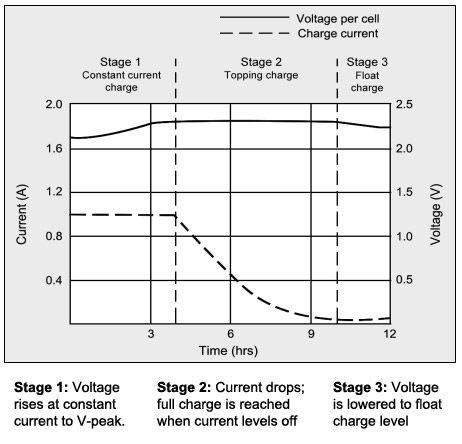
\includegraphics[width=7cm]{battery_charging.jpg}
    \caption{Lead Acid Battery Charging Cycle}
    \label{fig:battery_charging}
\end{figure}
\columnbreak The topping charge is essential for the well-being of the battery and can be compared to a little rest after a heavy meal. If continually deprived, the battery will eventually lose the ability to accept a full charge.The float charge in the third stage maintains the battery at full charge. The three stages are shown above in the figure1.
\section{Method}
\subsection{Components Used}
\begin{enumerate}
    \item AD620 Instrumentation Amplifier
    \item LF353 Operational Amplifier
    \item STP16N60M2 N-MOSFET
    \item Voltage Regulators - L7806, L7812, L7912 
    \item Capacitors - 1mF, 3.3nF, 0.1$\mu$F
    \item Inductors - 331$\mu$H
    \item Resistors - 47K$\Omega$, 100K$\Omega$, 10K$\Omega$, 100$\Omega$
    \item Power Resistors - 0.1$\Omega$ 5W
    \item Diodes - IN4001G
    \item Potentiometers - 100K$\Omega$, 10K$\Omega$
    \item Connectors
\end{enumerate}
List of other components used in the development stage are as follows:
\begin{itemize}
    \item Protoboard
    \item Digital Multimeter
    \item Function Generator
    \item Digital Oscilloscope
    \item Power Supply
    \item Various other passive components
\end{itemize}
\end{multicols}
\newpage
\begin{multicols}{2}
\subsubsection{AD620 Instrumentation\\Amplifier}
The AD620 is a low cost, high accuracy instrumentation amplifier that requires only one external resistor to set gains of 1 to 10,000. Furthermore, the AD620 features 8-lead SOIC and DIP packaging that is smaller than discrete designs and offers lower power (only 1.3 mA max supply current), making it a good fit for battery-powered, portable (or remote) applications. Furthermore, the low noise, low input bias current, and low power of the AD620 make it well suited for medical applications. In our design we used a potentiometer to set the gain to the desired value and to fine tune the gain in our desired range. We used instrumentation amplifier to give the feedback to the previous circuits.
\begin{figure}[H]
    \centering
    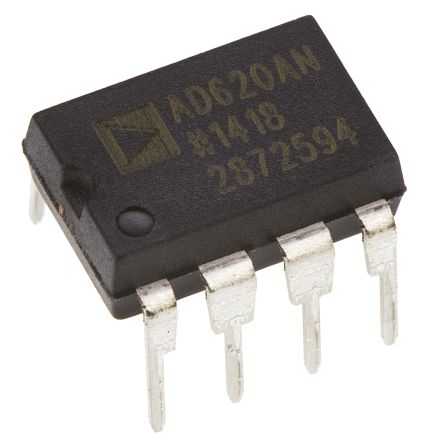
\includegraphics[width=7cm]{AD620.jpg}
    \caption{AD620 Instrumentation Amplifier}
    \label{fig:AD620}
\end{figure}
\subsubsection{LF353 Operational Amplifier}
These devices are low cost, high speed, dual JFET input operational amplifiers with an internally trimmed input offset voltage (BI-FET II technology). They require low supply current yet maintain a large gain bandwidth product and fast slew rate. \columnbreak In addition, well matched high voltage JFET input devices provide very low input bias and offset currents. These amplifiers may be used in applications such as
high speed integrators, fast D/A converters, sample and hold circuits and many other circuits. In our circuit to obtain high slew rate we used this operational amplifier instead of the typical LM741 operational amplifiers. 
\begin{figure}[H]
    \centering
    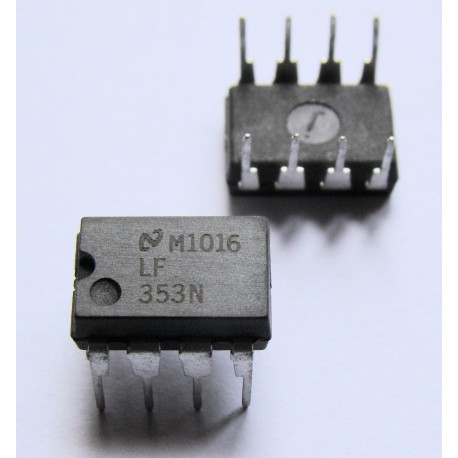
\includegraphics[width=7cm]{lf353.jpg}
    \caption{LF353 Operational Amplifier}
    \label{fig:LF353}
\end{figure}
\subsubsection{STP16N60M2 N-MOSFET}
These devices are N-channel Power MOSFETs developed using MDmesh™ M2 technology. Their strip layout and improved vertical structure, these devices exhibit low on-resistance and optimized switching characteristics, rendering them suitable for the most demanding high efficiency converters. Some of the features of this MOSFET are mentioned below.
\begin{figure}[H]
    \centering
    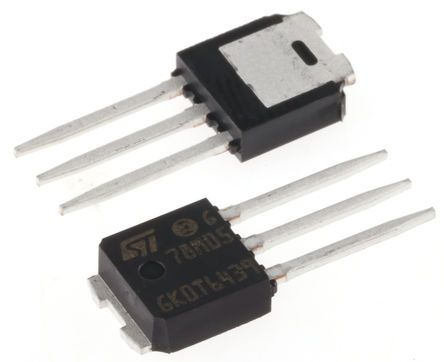
\includegraphics[width=5cm,height=4cm]{Mosfet.jpg}
    \caption{STP16N60M2 N-MOSFET}
    \label{fig:STP16N60M2 N-MOSFET}
\end{figure}
\end{multicols}
\begin{multicols}{2}
\begin{itemize}
    \item Extremely low gate charge
    \item Excellent output capacitance (C$_{OSS}$) profile
    \item 100\% avalanche tested
    \item Zener-protected
\end{itemize}
\subsubsection{Hardware Development}
There are many ways to implement a Constant Current Source for battery charging but the challenge that we have to face here was to implement a current source with low power consumption. In order to do that we have to reduce unwanted power losses in our circuit. In order to implement the final circuit, we had to go through a lot of experimental circuits. Not only that, we had to consider the availability of the components of the circuits. In our projects, there are mainly 4 stages.
\begin{enumerate}
    \item Ramp wave generator
    \item Comparator(for Pulse Width Modulation)
    \item Buck Converter
    \item Amplifier
\end{enumerate}
We generate a ramp wave using the Ramp wave generator and get an adjustable rectangular wave form using the comparator.  After that we get a constant voltage by supplying that rectangular wave form through the buck converter for charging the battery. In order to get the current through the battery to be constant, we use a shunt series resistant to the battery and get a voltage feedback proportional to the battery voltage and amplify it through the amplifier circuit. Then that voltage is supplied to the comparator as a feedback signal. By adjusting the amplification factor, we can get the current through the battery constant. For the amplifier circuit, we used an instrumentation amplifier AD620.
\subsubsubsection{Ramp Generating Circuit}
The purpose of generating this ramp signal is to generate a PWM signal. In order to do that, we have to get an adjustable rectangular wave and in order to accomplish that we use the aforementioned ramp signal. Even though we came up with several number of ramp circuits, the problem was to implement a power efficient Ramp circuit. To do that we have to remove the transistors due to the high-power dissipation. In the final ramp generator, a rectangular wave form is generated and by using an integrator, we integrate it and get the ramp waveform.
\subsubsubsection{Comparator (for PWM)}
In this stage we compare the ramp circuit signal with the feedback of the buck converter through the instrumentation amplifier in order to adjust the pulse width of the rectangular waveform. This was done to vary the voltage deference across the battery with the increment of the battery voltage. Therefore, the current through the battery is always constant.
\subsubsubsection{Buck Converter}
We use the rectangular wave output of the comparator as a switch to the buck converter and hence the voltage supplied to the buck converter is also a rectangular pulse and eventually the output is the DC voltage that we need to charge. By varying the positive cycle width of the input rectangular pulse, the output DC voltage can be varied.
\subsubsubsection{Amplifier}
In order to vary the voltage across the battery, feedback from the battery voltage has to be taken out. So that the voltage across the shunt resistor is amplified by an AD620 instrumentation amplifier and input it to the comparator.\\\\
After all these stages are interconnected, when battery is plugged in, the voltage in the battery and voltage deference across the battery is being increased due to the charging and the current through the battery will be constant. After charging is completed, the voltage rising of the battery will be stopped, Therefore the feedback will be constant and the voltage deference across the battery remains constant. Hence, after battery is fully charged, the constant current source is automatically act as the constant voltage source.\\
All the relevant circuits are mentioned in the appendices.
\subsubsection{Testing \& Fabricating PCBs}
Before making the PCBs all the circuits were thoroughly tested on bread board to make sure the functionality of those circuits. As the full circuit consists of three major sub parts; a separate PCB for each part have been designed. Track widths of the PCB of the Buck converter circuit were kept wider as a high current flow through that circuit. All the PCBs were designed using the Altium\textsuperscript{\textregistered} software. Therefore, the 3D view of the PCBs was considered to organize the components on the PCBs in a proper way.
\begin{figure}[H]
    \centering
    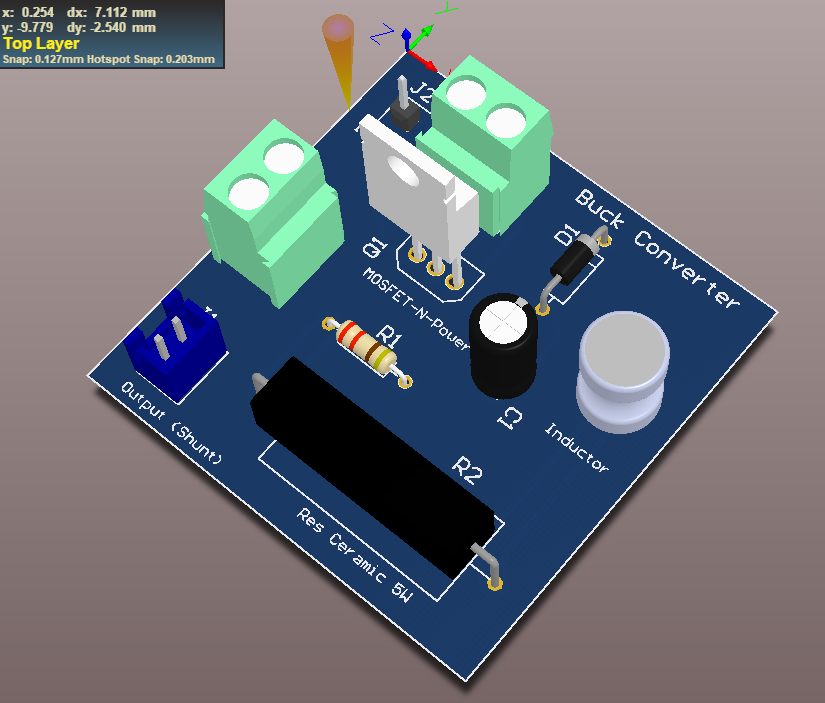
\includegraphics[width=7cm]{Fig_01.png}
    \caption{Buck Converter in 3D view}
    \label{fig:Buck Converter in 3D view}
\end{figure}
PCBs were manufactured by the JLCPCB\textsuperscript{\textregistered} in China. Mounting components were done after arriving the PCBs and all the connections were carefully checked several times to make sure the functionality of the PCBs.
\begin{figure}[H]
    \centering
    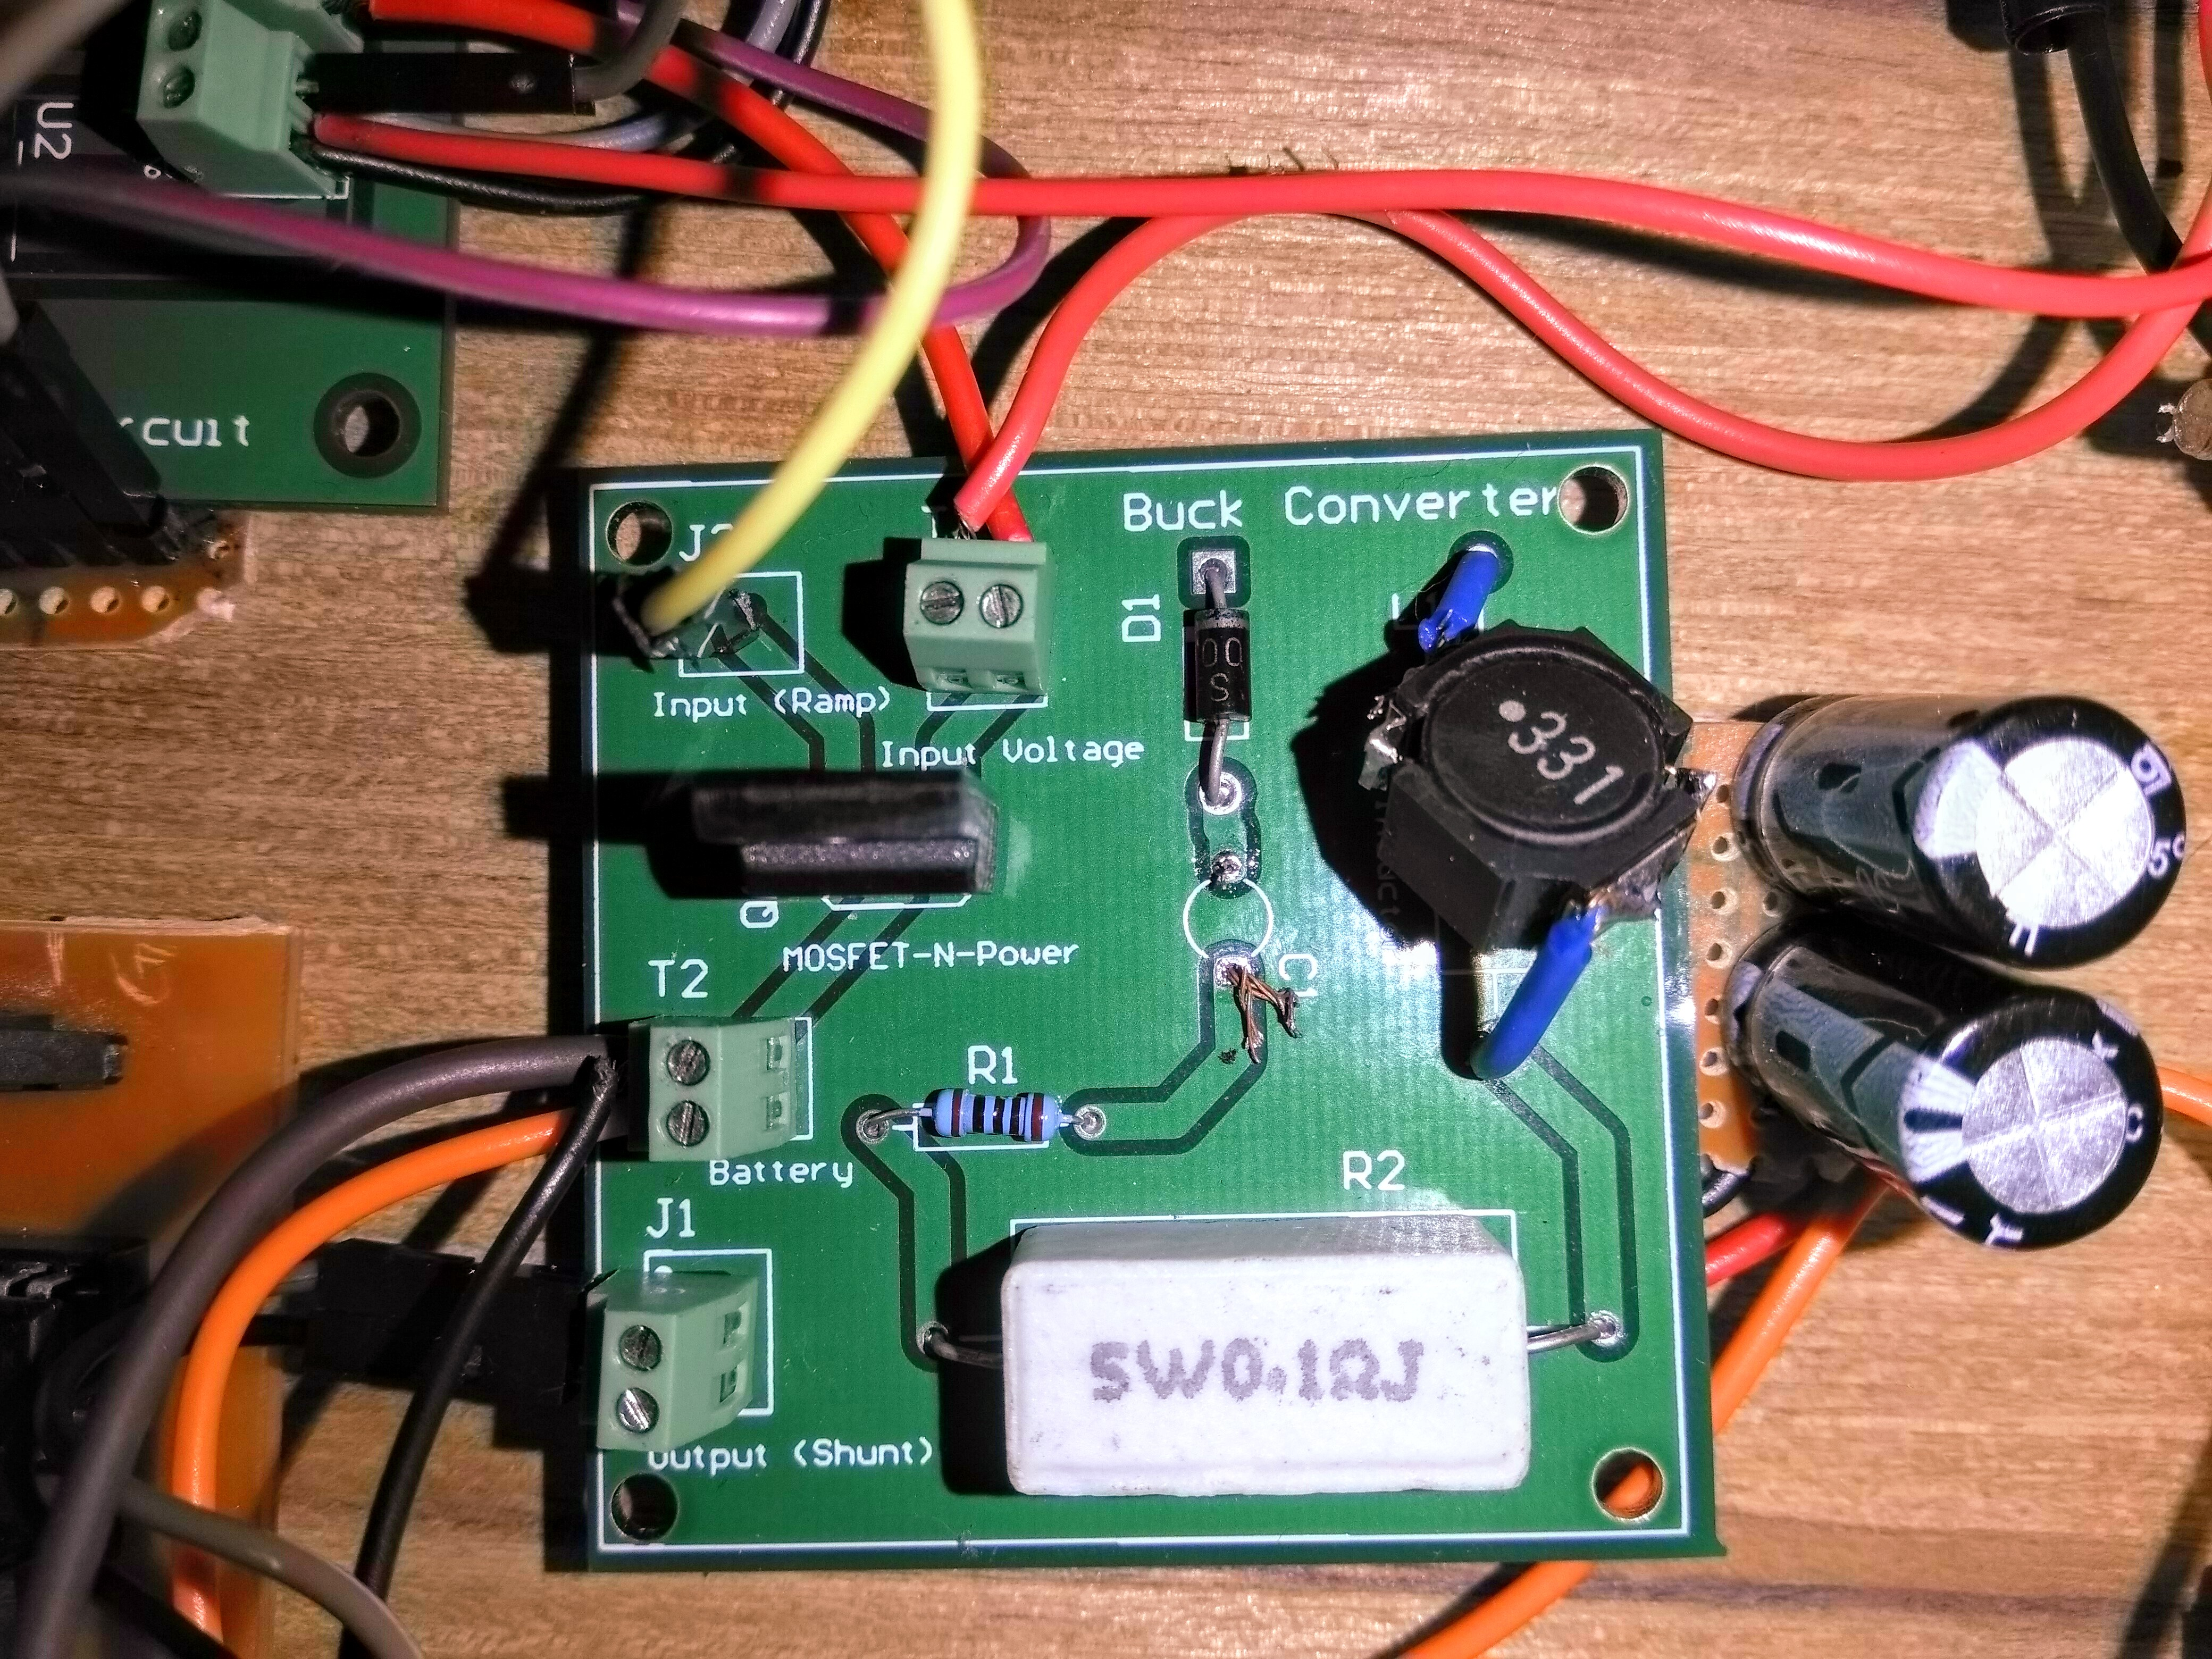
\includegraphics[width=7cm]{Fig_02.jpeg}
    \caption{Buck Converter}
    \label{fig:PWM signal Generator}
\end{figure}
\begin{figure}[H]
    \centering
    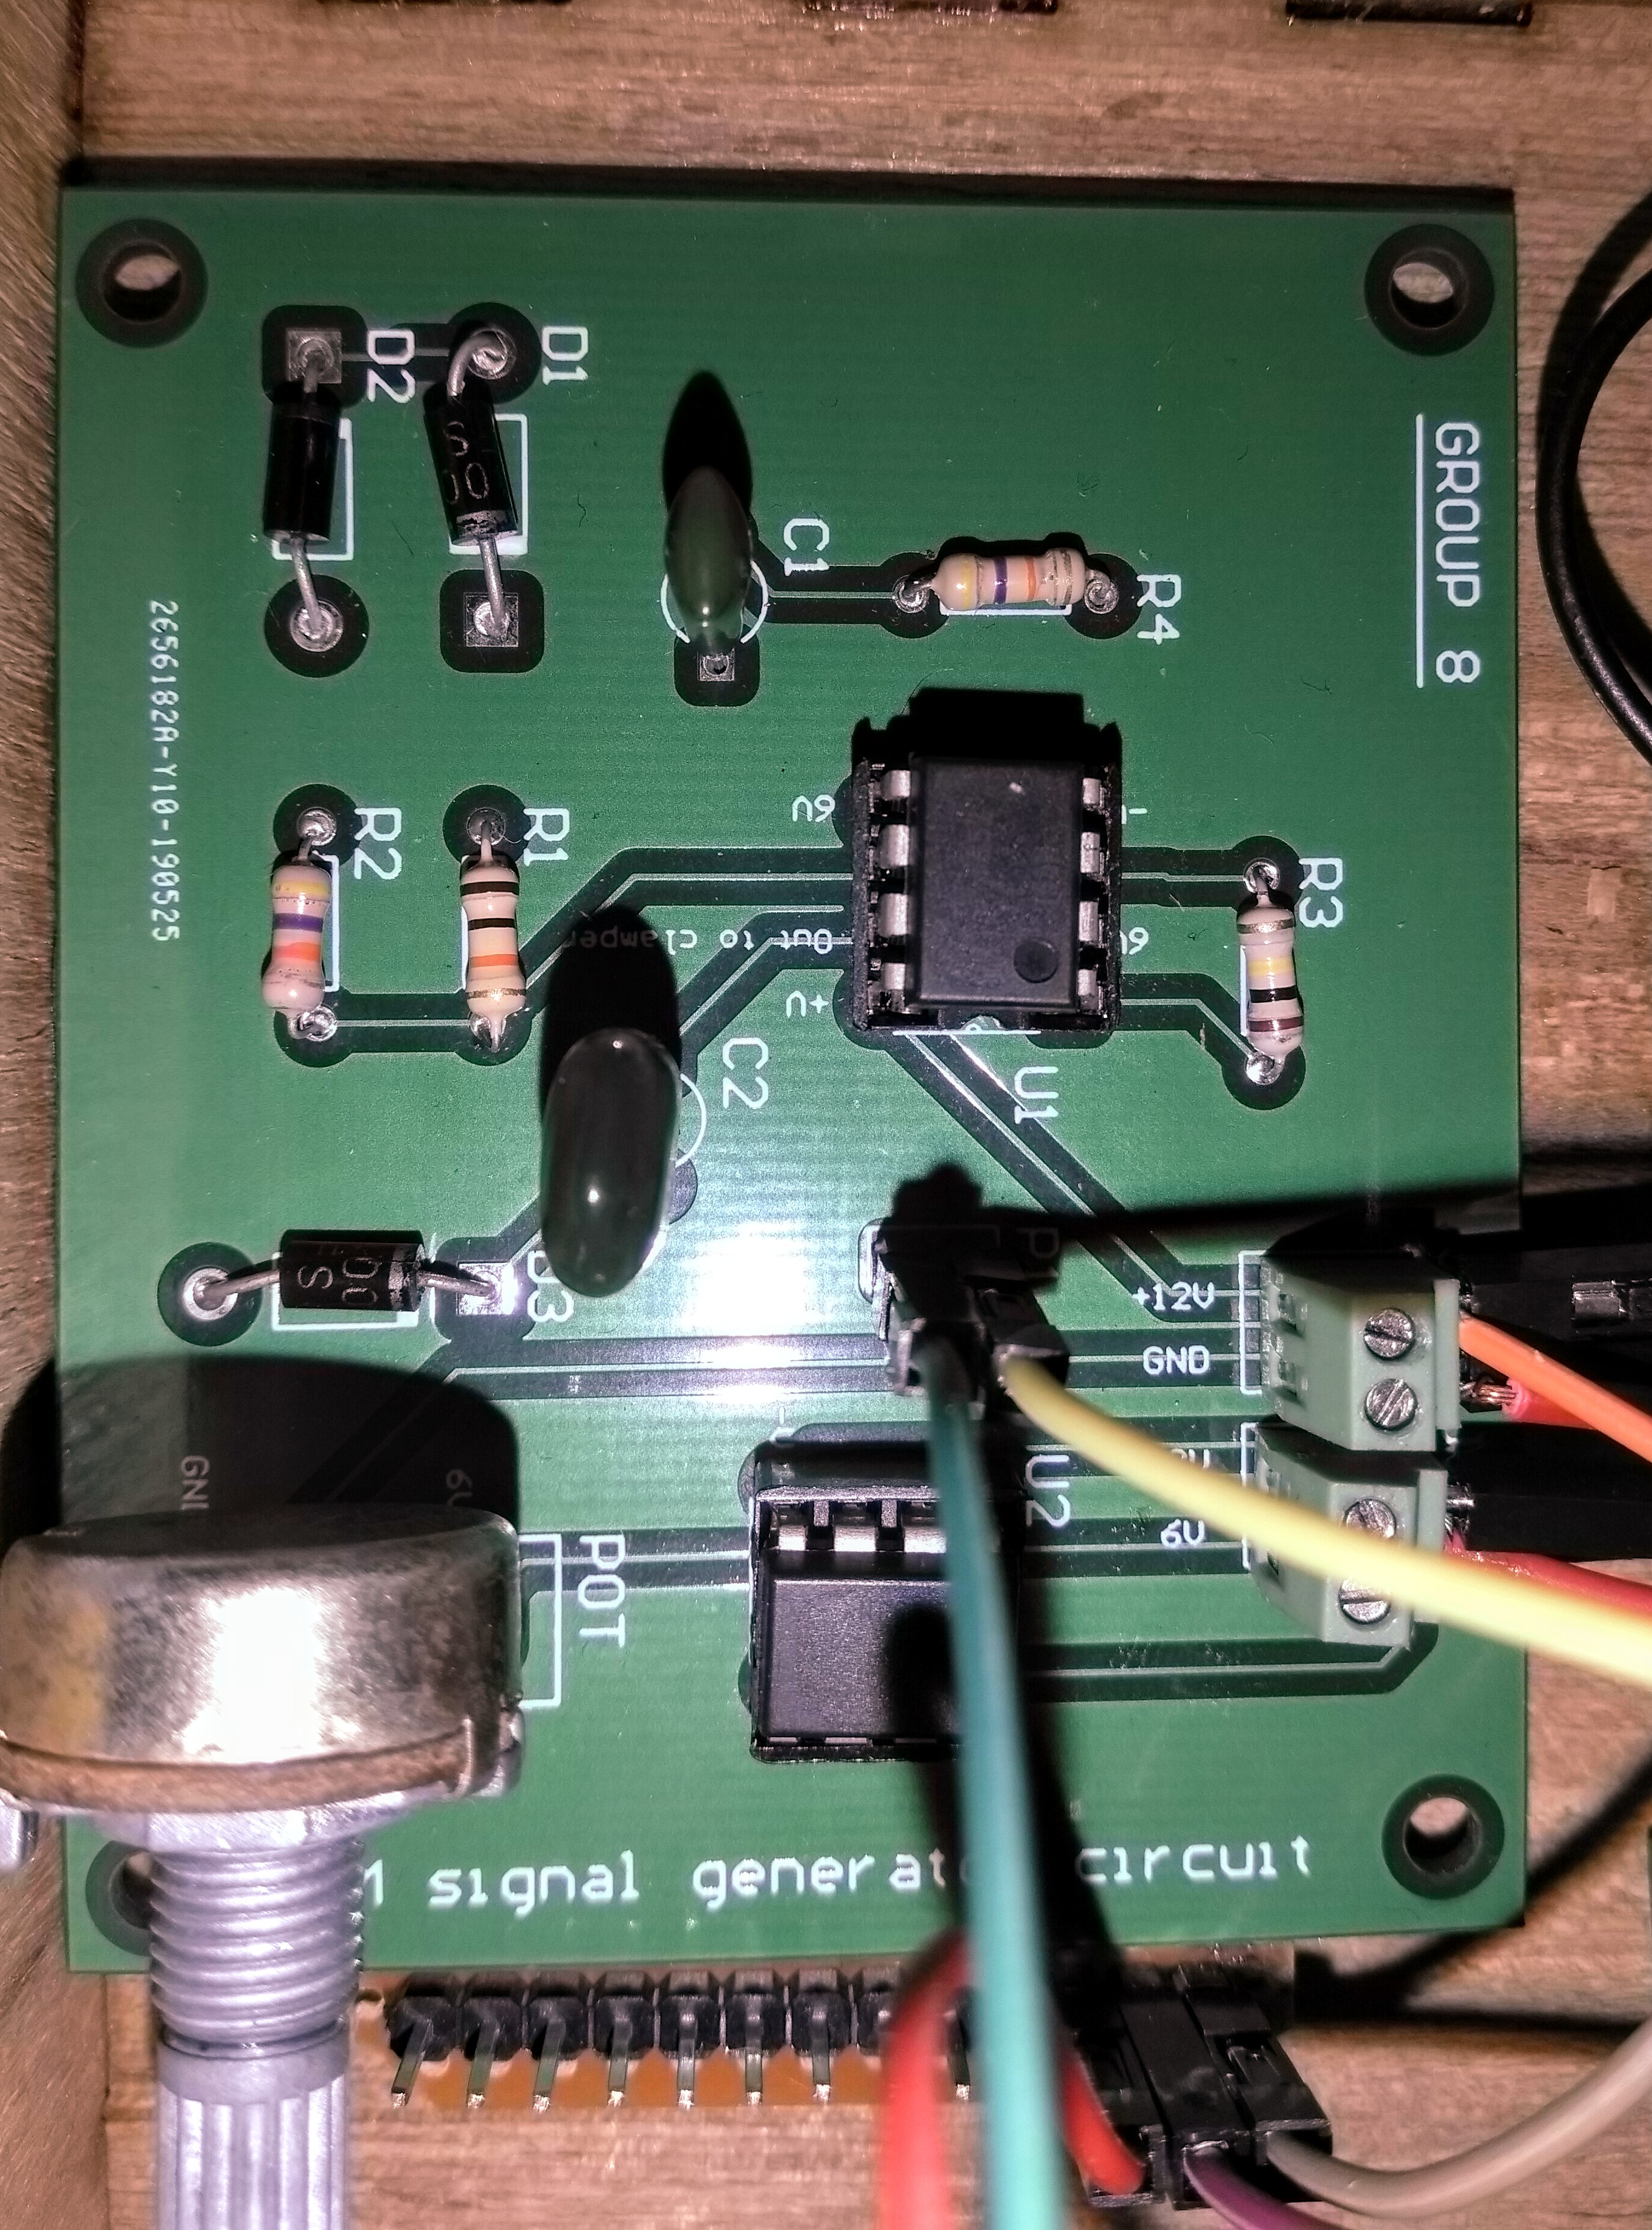
\includegraphics[width=7cm]{Fig_03.jpg}
    \caption{PWM signal Generator}
    \label{fig:Buck Converter}
\end{figure}
\subsubsection{Enclosure Design}
According to the project guideline the enclosure design was a main part and in order to do that we used SolidWorks\textsuperscript{\textregistered} 3D modelling software and chose material as wood. All the enclosure designing was done by laser cutting. To measure the current through the load and the voltage across the load we used two separate Ammeter and Voltmeter in the enclosure design.
\begin{figure}[H]
    \centering
    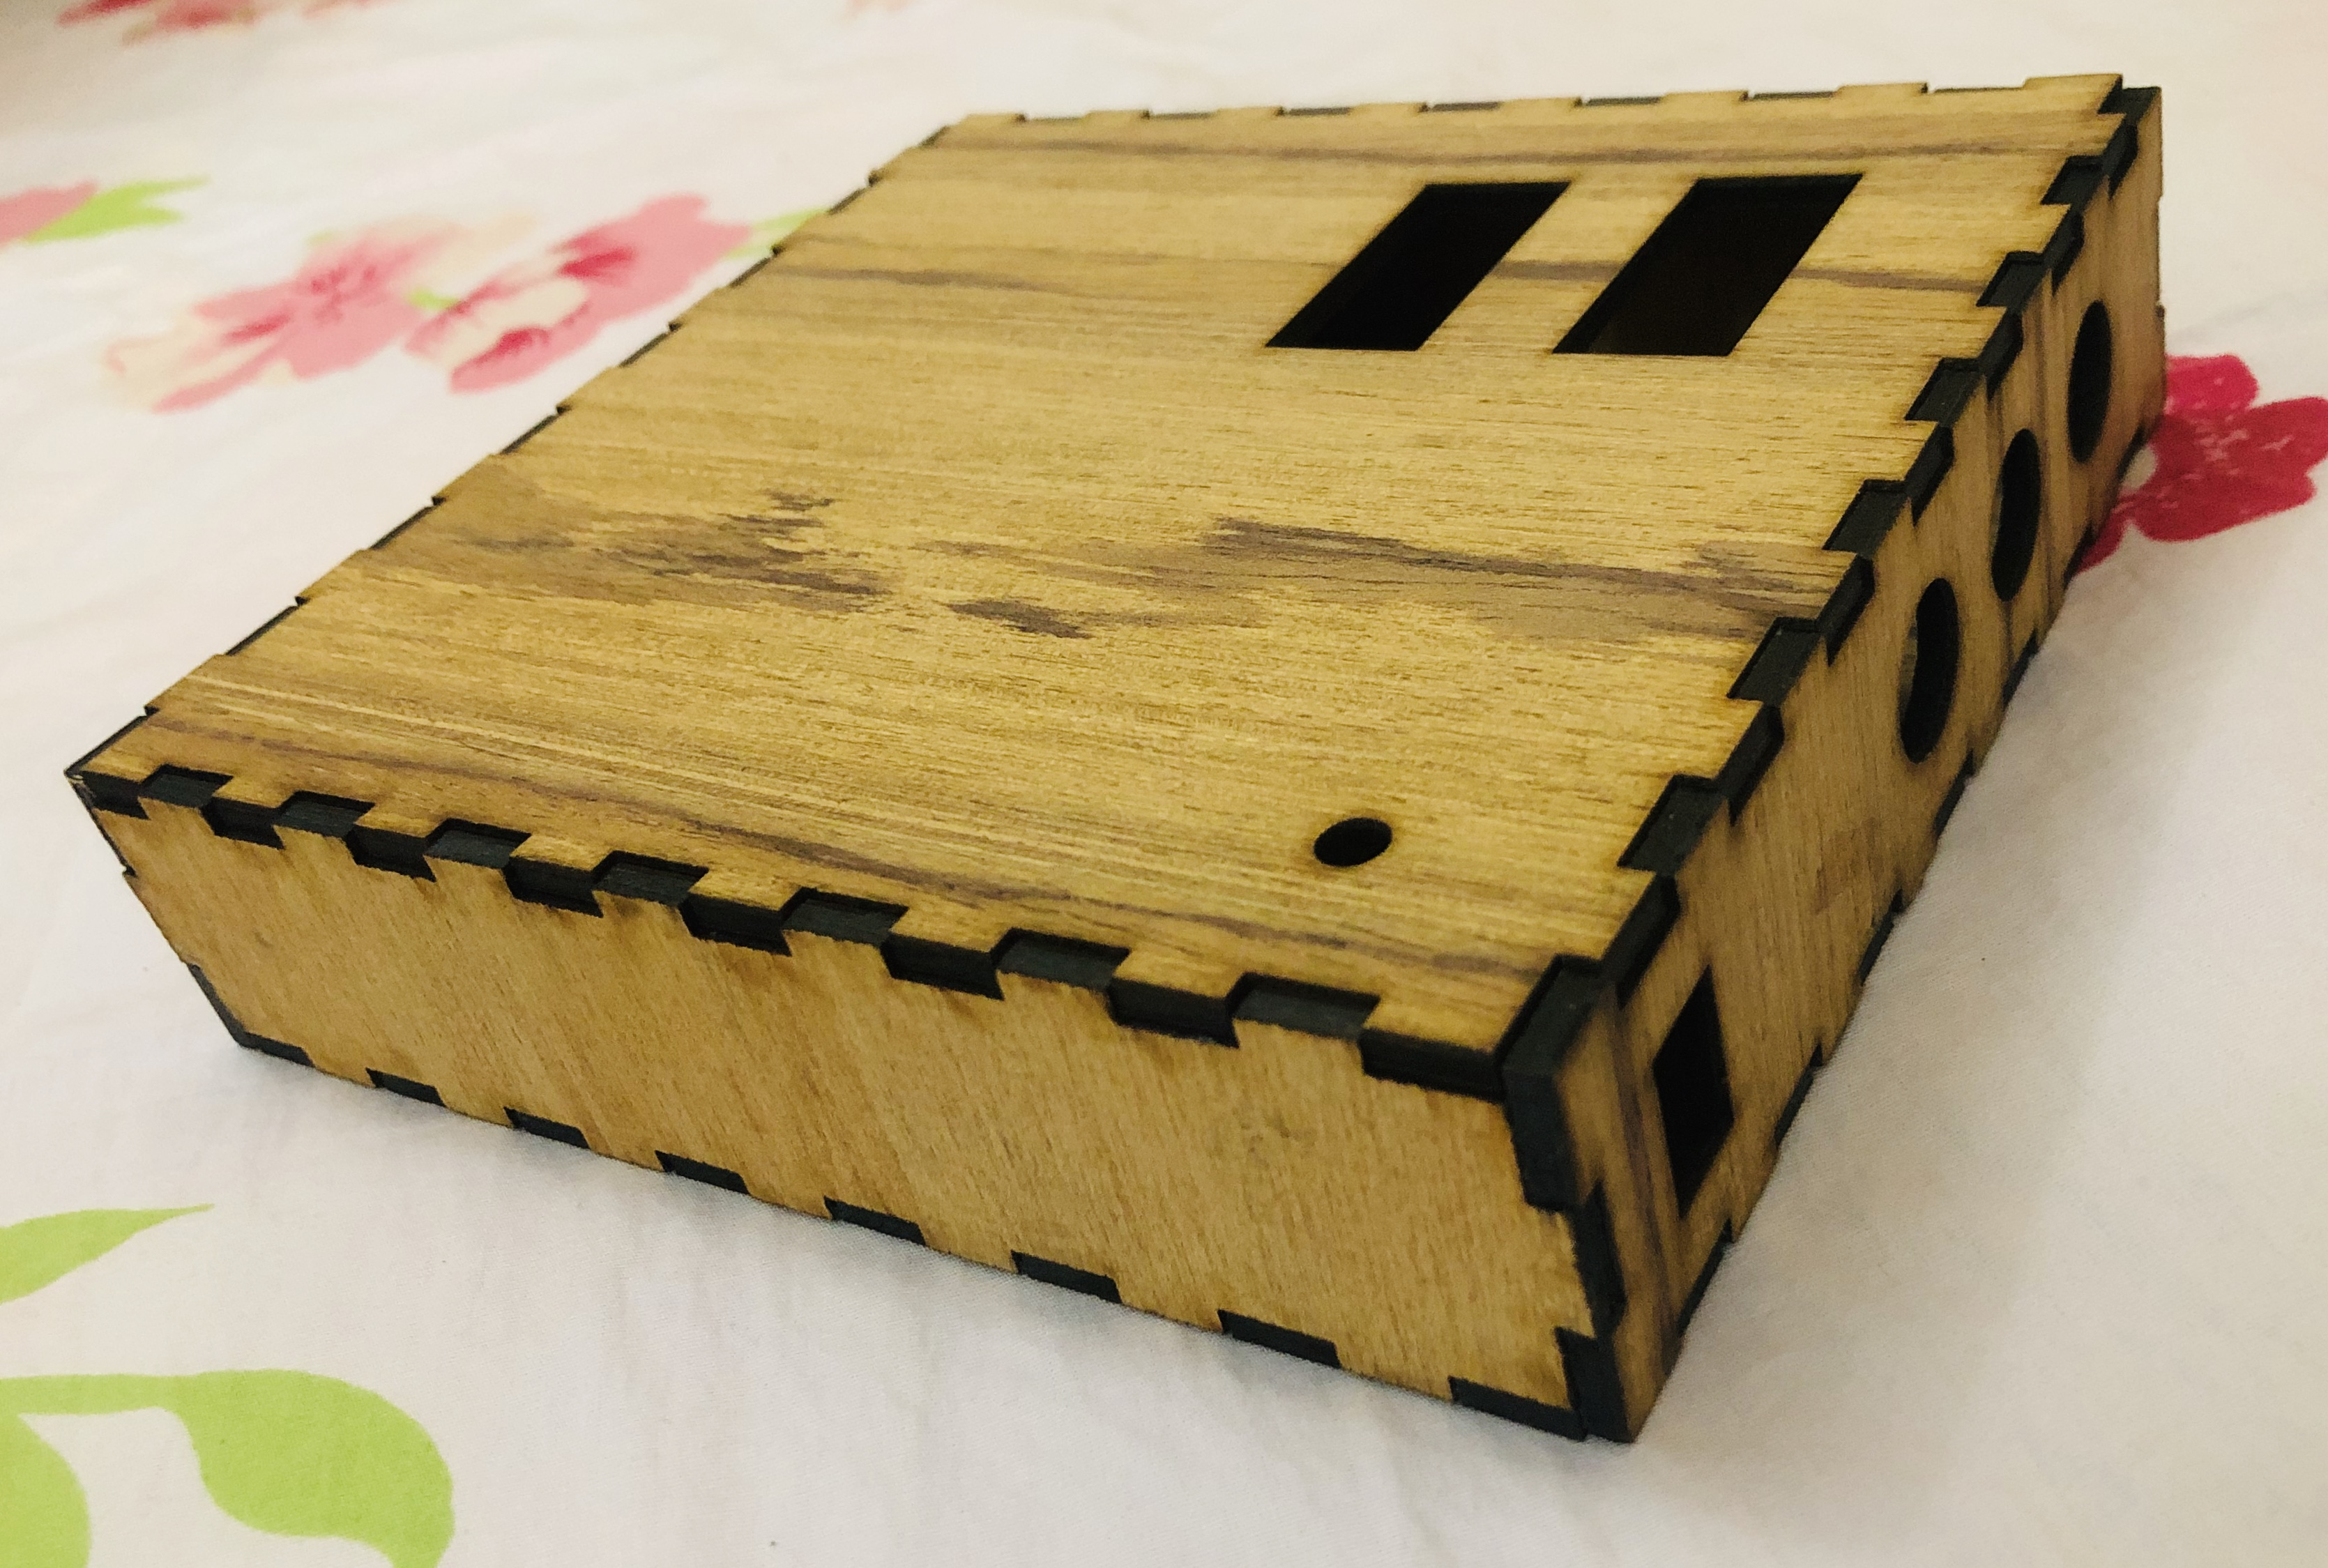
\includegraphics[width=7cm]{enclosure1.jpg}
    \caption{Enclosure Design}
    \label{fig:Enclosure}
\end{figure}
\section{Results}
The following figures show the simulation results and the results we obtained when testing the circuit using a bread board. Operational Amplifiers have been used as the main components of the circuit to minimize the power dissipation.
Circuit has a feedback given from the shunt resistor to the comparator to keep the current constant even when the battery voltage increases. Different voltages levels were given by using different high power rated ceramic resistors as an alternative for a battery and the overall functionality of the system was tested. In fact, each time circuit gave the required constant 1A current to the load (ceramic resistor) which represents the battery.
\begin{figure}[H]
    \centering
    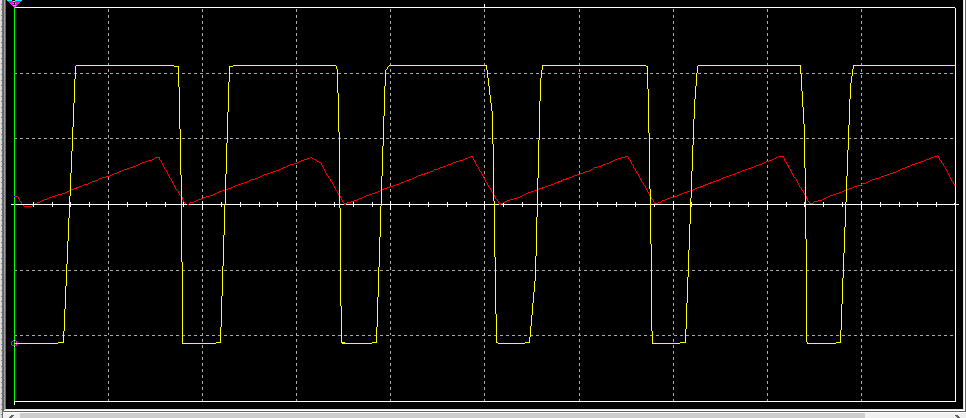
\includegraphics[width=7cm]{Ramp_PWM.png}
    \caption{Ramp and PWM Signal}
    \label{fig:Ramp_PWM_Result}
\end{figure}
\begin{figure}[H]
    \centering
    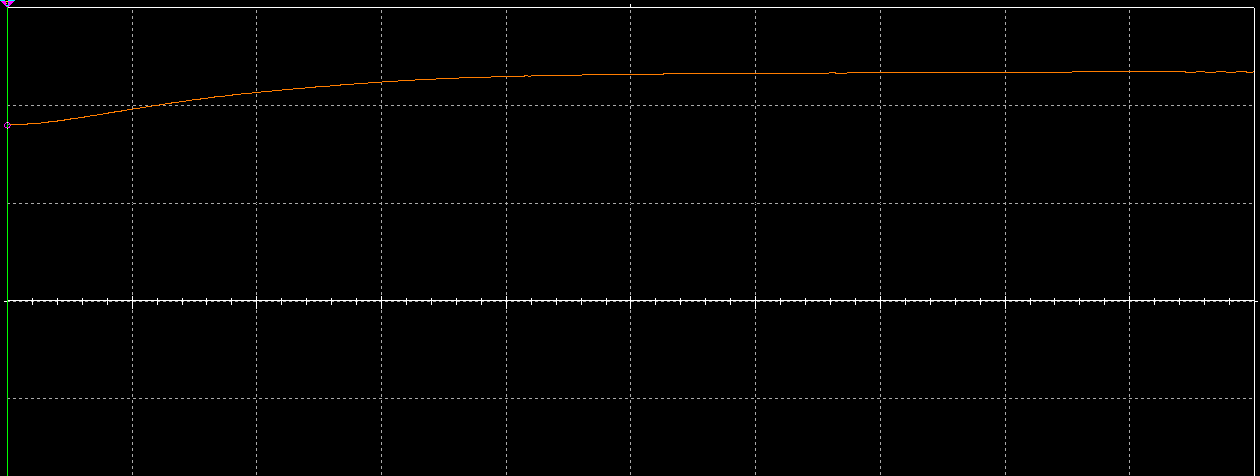
\includegraphics[width=7cm]{const_voltage.png}
    \caption{Constant Voltage across Shunt Resistor}
    \label{fig:Ramp_PWM}
\end{figure}
\begin{figure}[H]
    \centering
    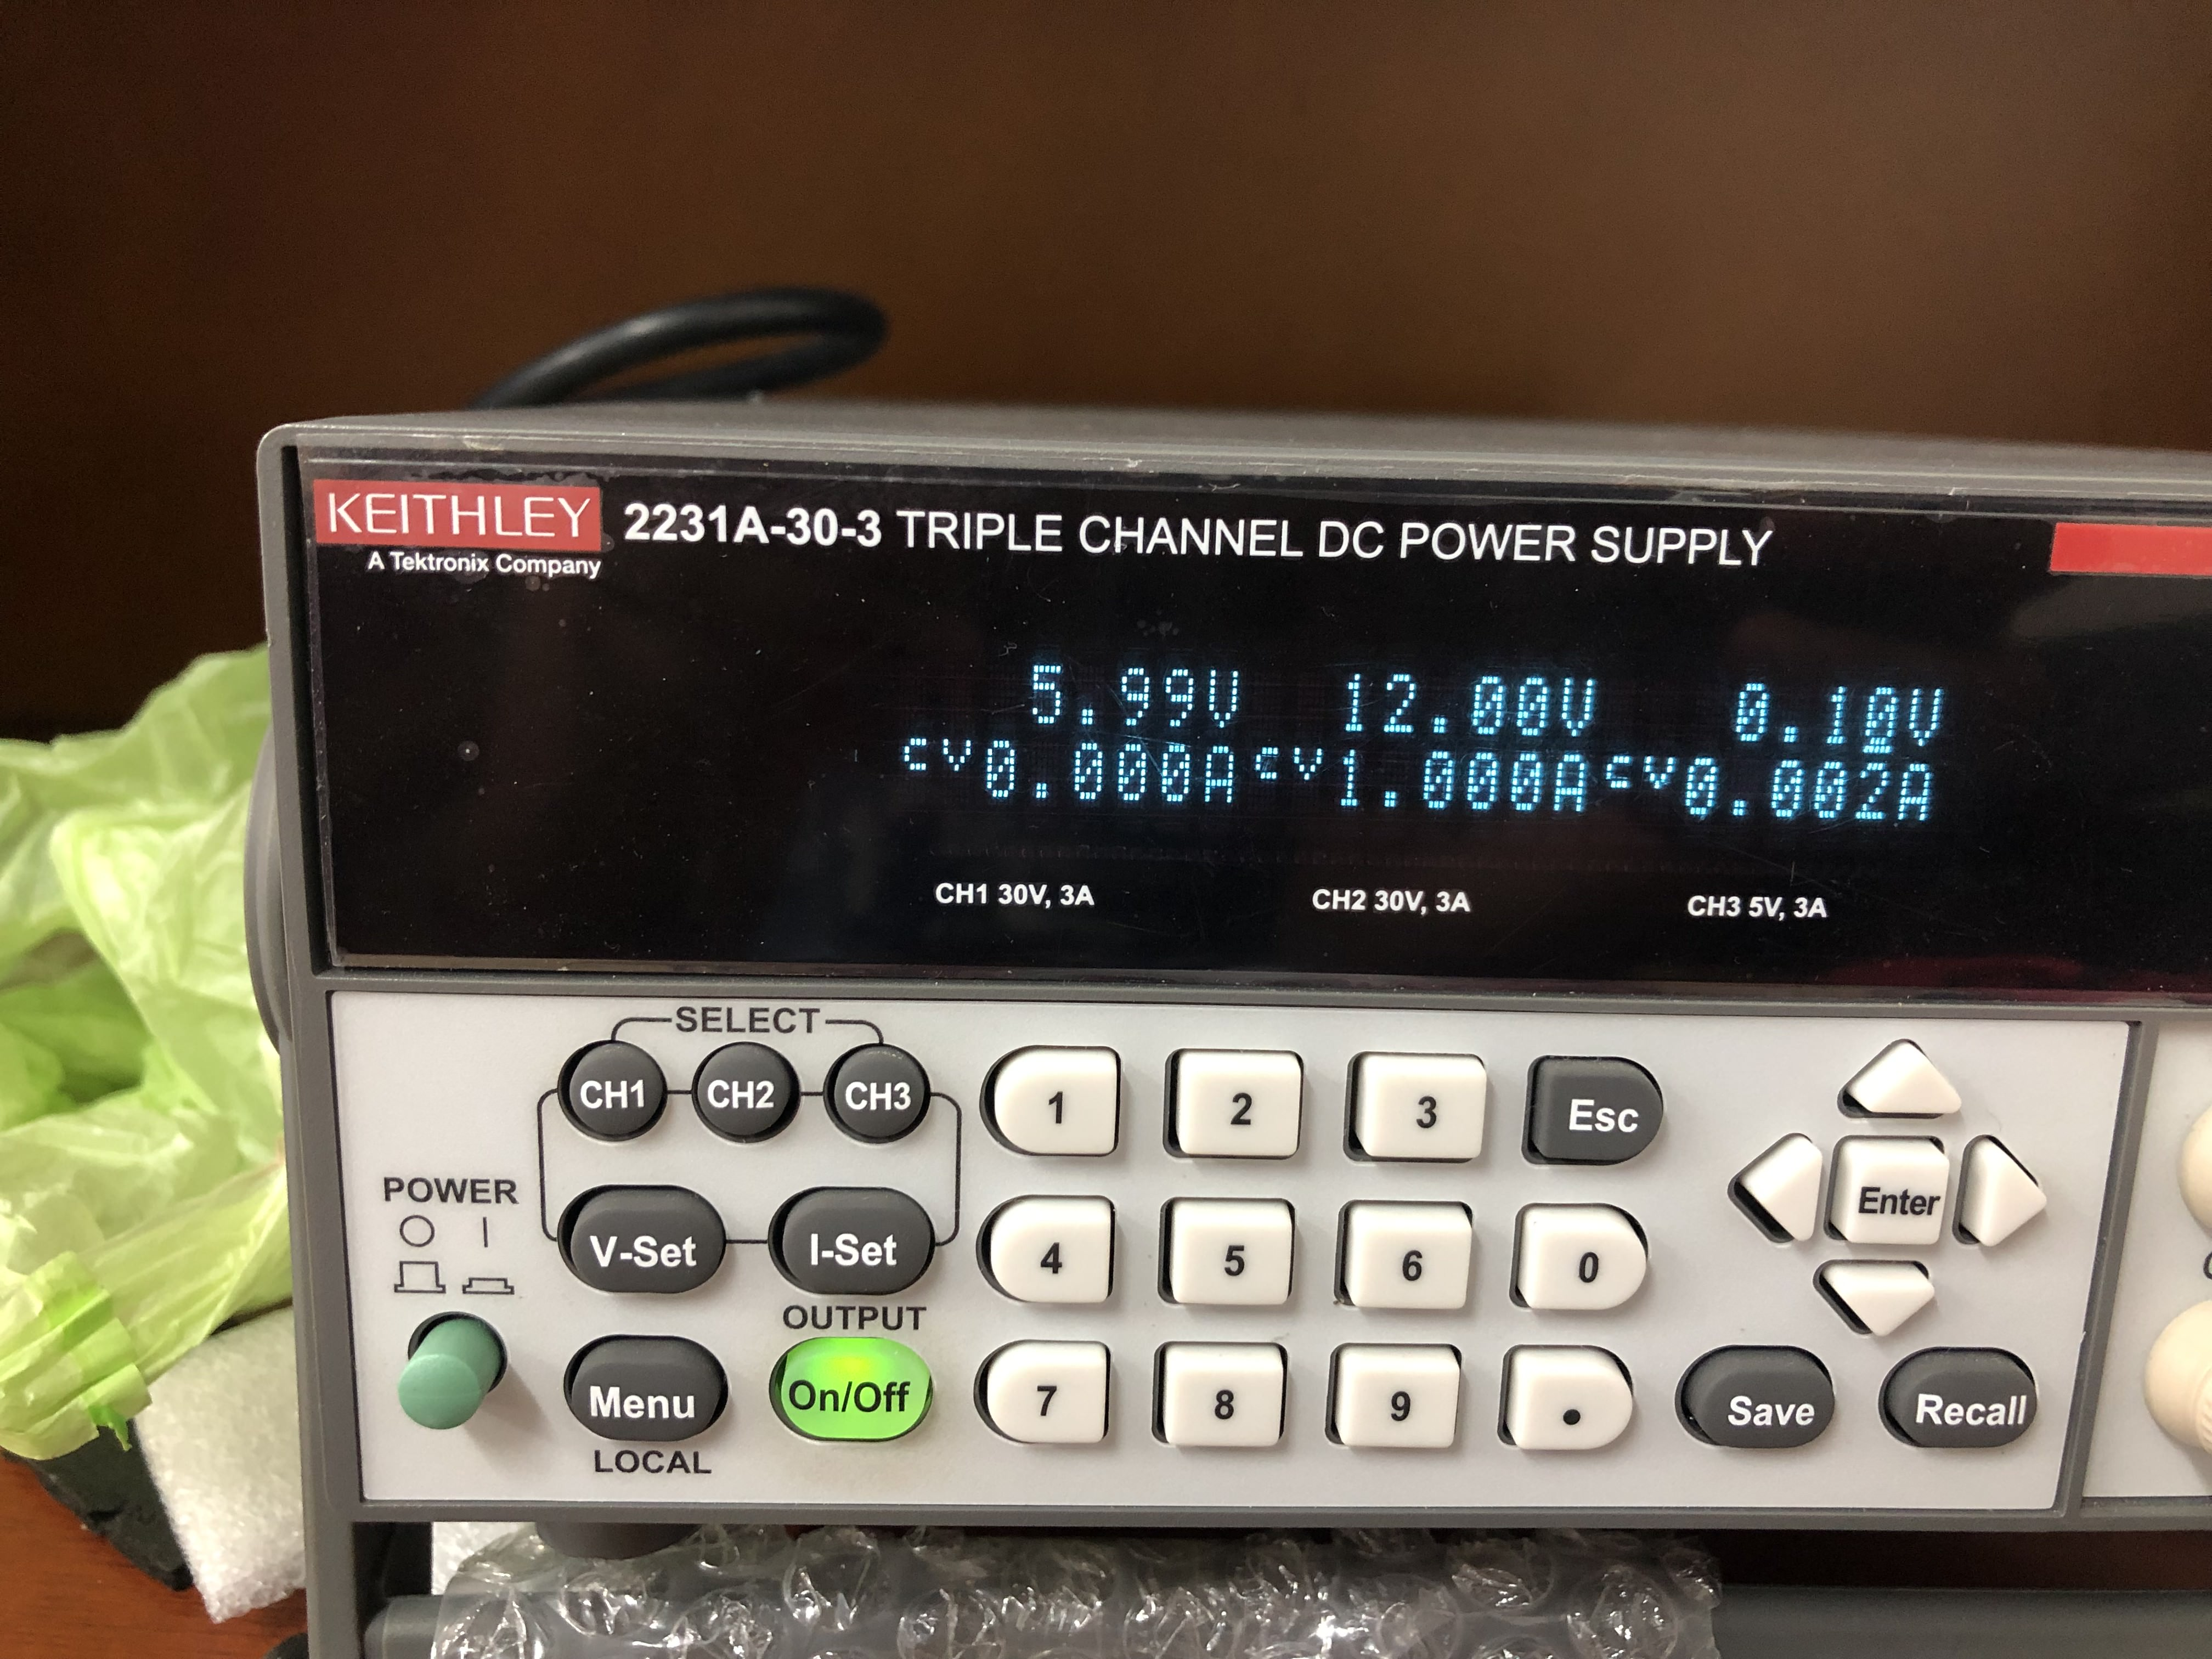
\includegraphics[width=7cm]{1A_current.jpg}
    \caption{1A current flows through the Buck Converter}
    \label{fig:1A current flows through the Buck circuit}
\end{figure}
\begin{figure}[H]
    \centering
    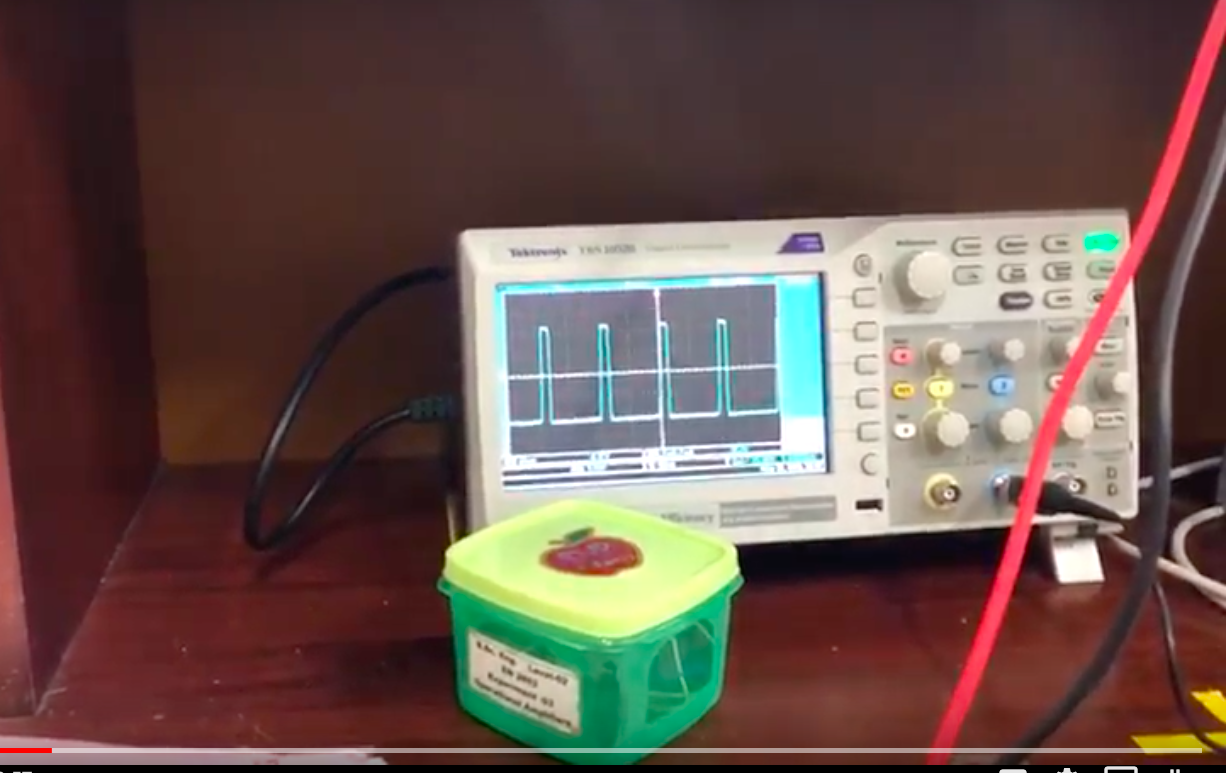
\includegraphics[width=7cm]{PWM_Signal.png}
    \caption{PWM signal}
    \label{fig:PWM_signal_result}
\end{figure}
\section{Discussion}
Obtaining a constant current of 1A to charge a 12V lead acid battery was the main goal of our project. Usual implementations of constant current sources consist of transistors which results in high heat dissipation and thus a larger power loss. Therefore, we addressed this problem by building a circuit entirely of operational amplifiers. Maintaining a constant current across the load was done by the use of a feedback circuit which measures the voltage across a fixed(constant) resistor in series with the load, amplifies it using an instrumentation amplifier and feeds it to the OpAmp used as a comparator, to generate the PWM signal which is then forwarded to a buck converter to produce the required voltage across the load, thus maintaining a constant current of 1A.\\
The generated ramp signal for the comparator had a minor DC shift. Even though, we managed to clamp this signal in the software simulation, practically when we cascaded all the different stages together, we observed that this shift differed each time. Therefore, after powering up the whole circuit we had to always adjust R$_g$ of the instrumentation amplifier and make sure the feedback voltage falls within the voltage range of the ramp signal. As an improvement, with the addition of 2-3 more stages in the feedback circuit, the output of this device will be more accurate, and it will be more convenient for the end user to handle.\\
Furthermore, we specially used a buck converter to generate the required voltage and current from the PWM signal and an instrumentation amplifier for voltage amplification to ensure maximum isolation of circuits so that the output of one stage will not change drastically when they are cascaded.
\section{Acknowledgement}
We would like to express our gratitude to our supervisor Mr.Thilina Ambagahawaththa, who took keen interest in our project work and guided us all along, till the completion of our project work. Our sincere thanks go to Mr.Asanka Rathnayake as well for the technical advice and guidance given
We pay our gratitude to the rest of the academic staff who intimately welcomed us to share their knowledge and experiences. We are very grateful to the personnel who are in charge of laboratories for allowing us to use the laboratories when needed and for the support given to solve technical issues.\\
Softwares Used:
\begin{itemize}
    \item Altium Designer\textsuperscript{\textregistered} 2017
    \item SolidWorks\textsuperscript{\textregistered} 2018
    \item AutoCAD\textsuperscript{\textregistered} 2018
\end{itemize}
\end{multicols}
\section{References}
\begin{enumerate}
    \item https://www.electronics-tutorial.net/analog-integrated-circuits/multivibrators/sawtooth-waveform-generator/
    \item https://www.elprocus.com/sawtooth-wave-generator-and-its-working-principle/
    \item https://circuitdigest.com/electronic-circuits/sawtooth-waveform-generator-circuit-using-op-amp
    \item http://www.ti.com/lit/ds/symlink/lf353-n.pdf
    \item https://www.mouser.com/ProductDetail/STMicroelectronics/STP16N60M2?qs=fGtbh\\\%252BGvP67tkTXdaZuqIg\%3D\%3D
    \item https://www.analog.com/media/en/technical-documentation/data-sheets/AD620.pdf
    \item http://www.learnabout-electronics.org/PSU/psu31.php
\end{enumerate}
\newpage
\section{Appendices}
\subsection{Circuit Designs}
\begin{figure}[h]
    \centering
    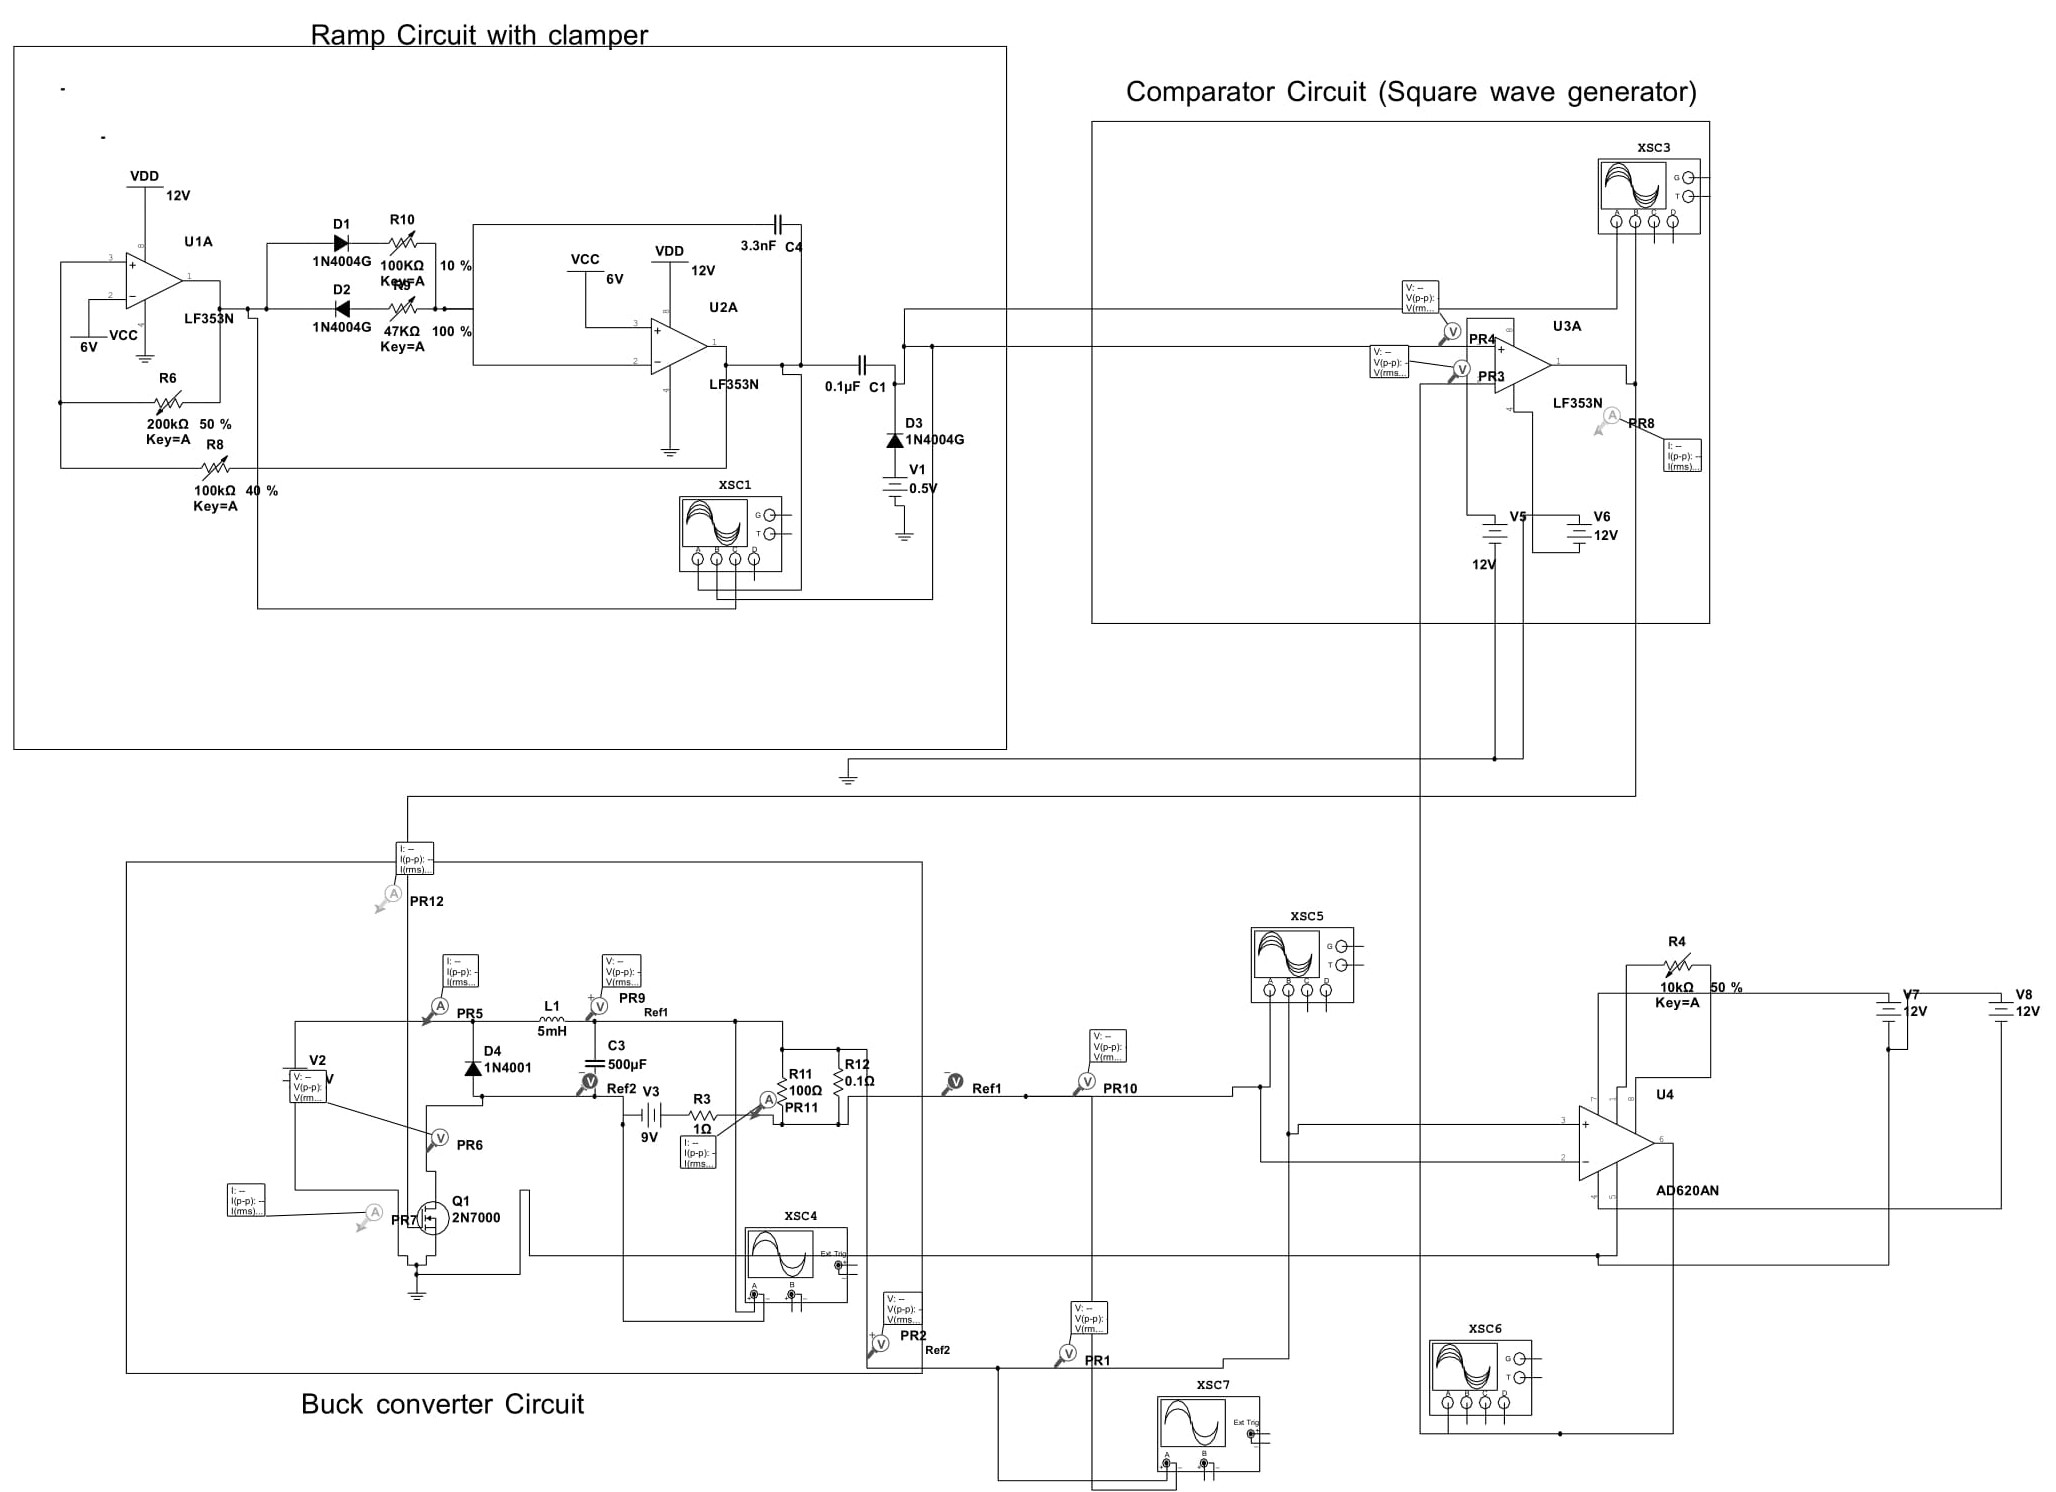
\includegraphics[angle=270,origin=c,scale=0.337]{Fig_04-1.jpg}
    \caption{Overall Circuit}
    \label{fig:Overall Circuit}
\end{figure}
\newpage
\begin{figure}[H]
    \centering
    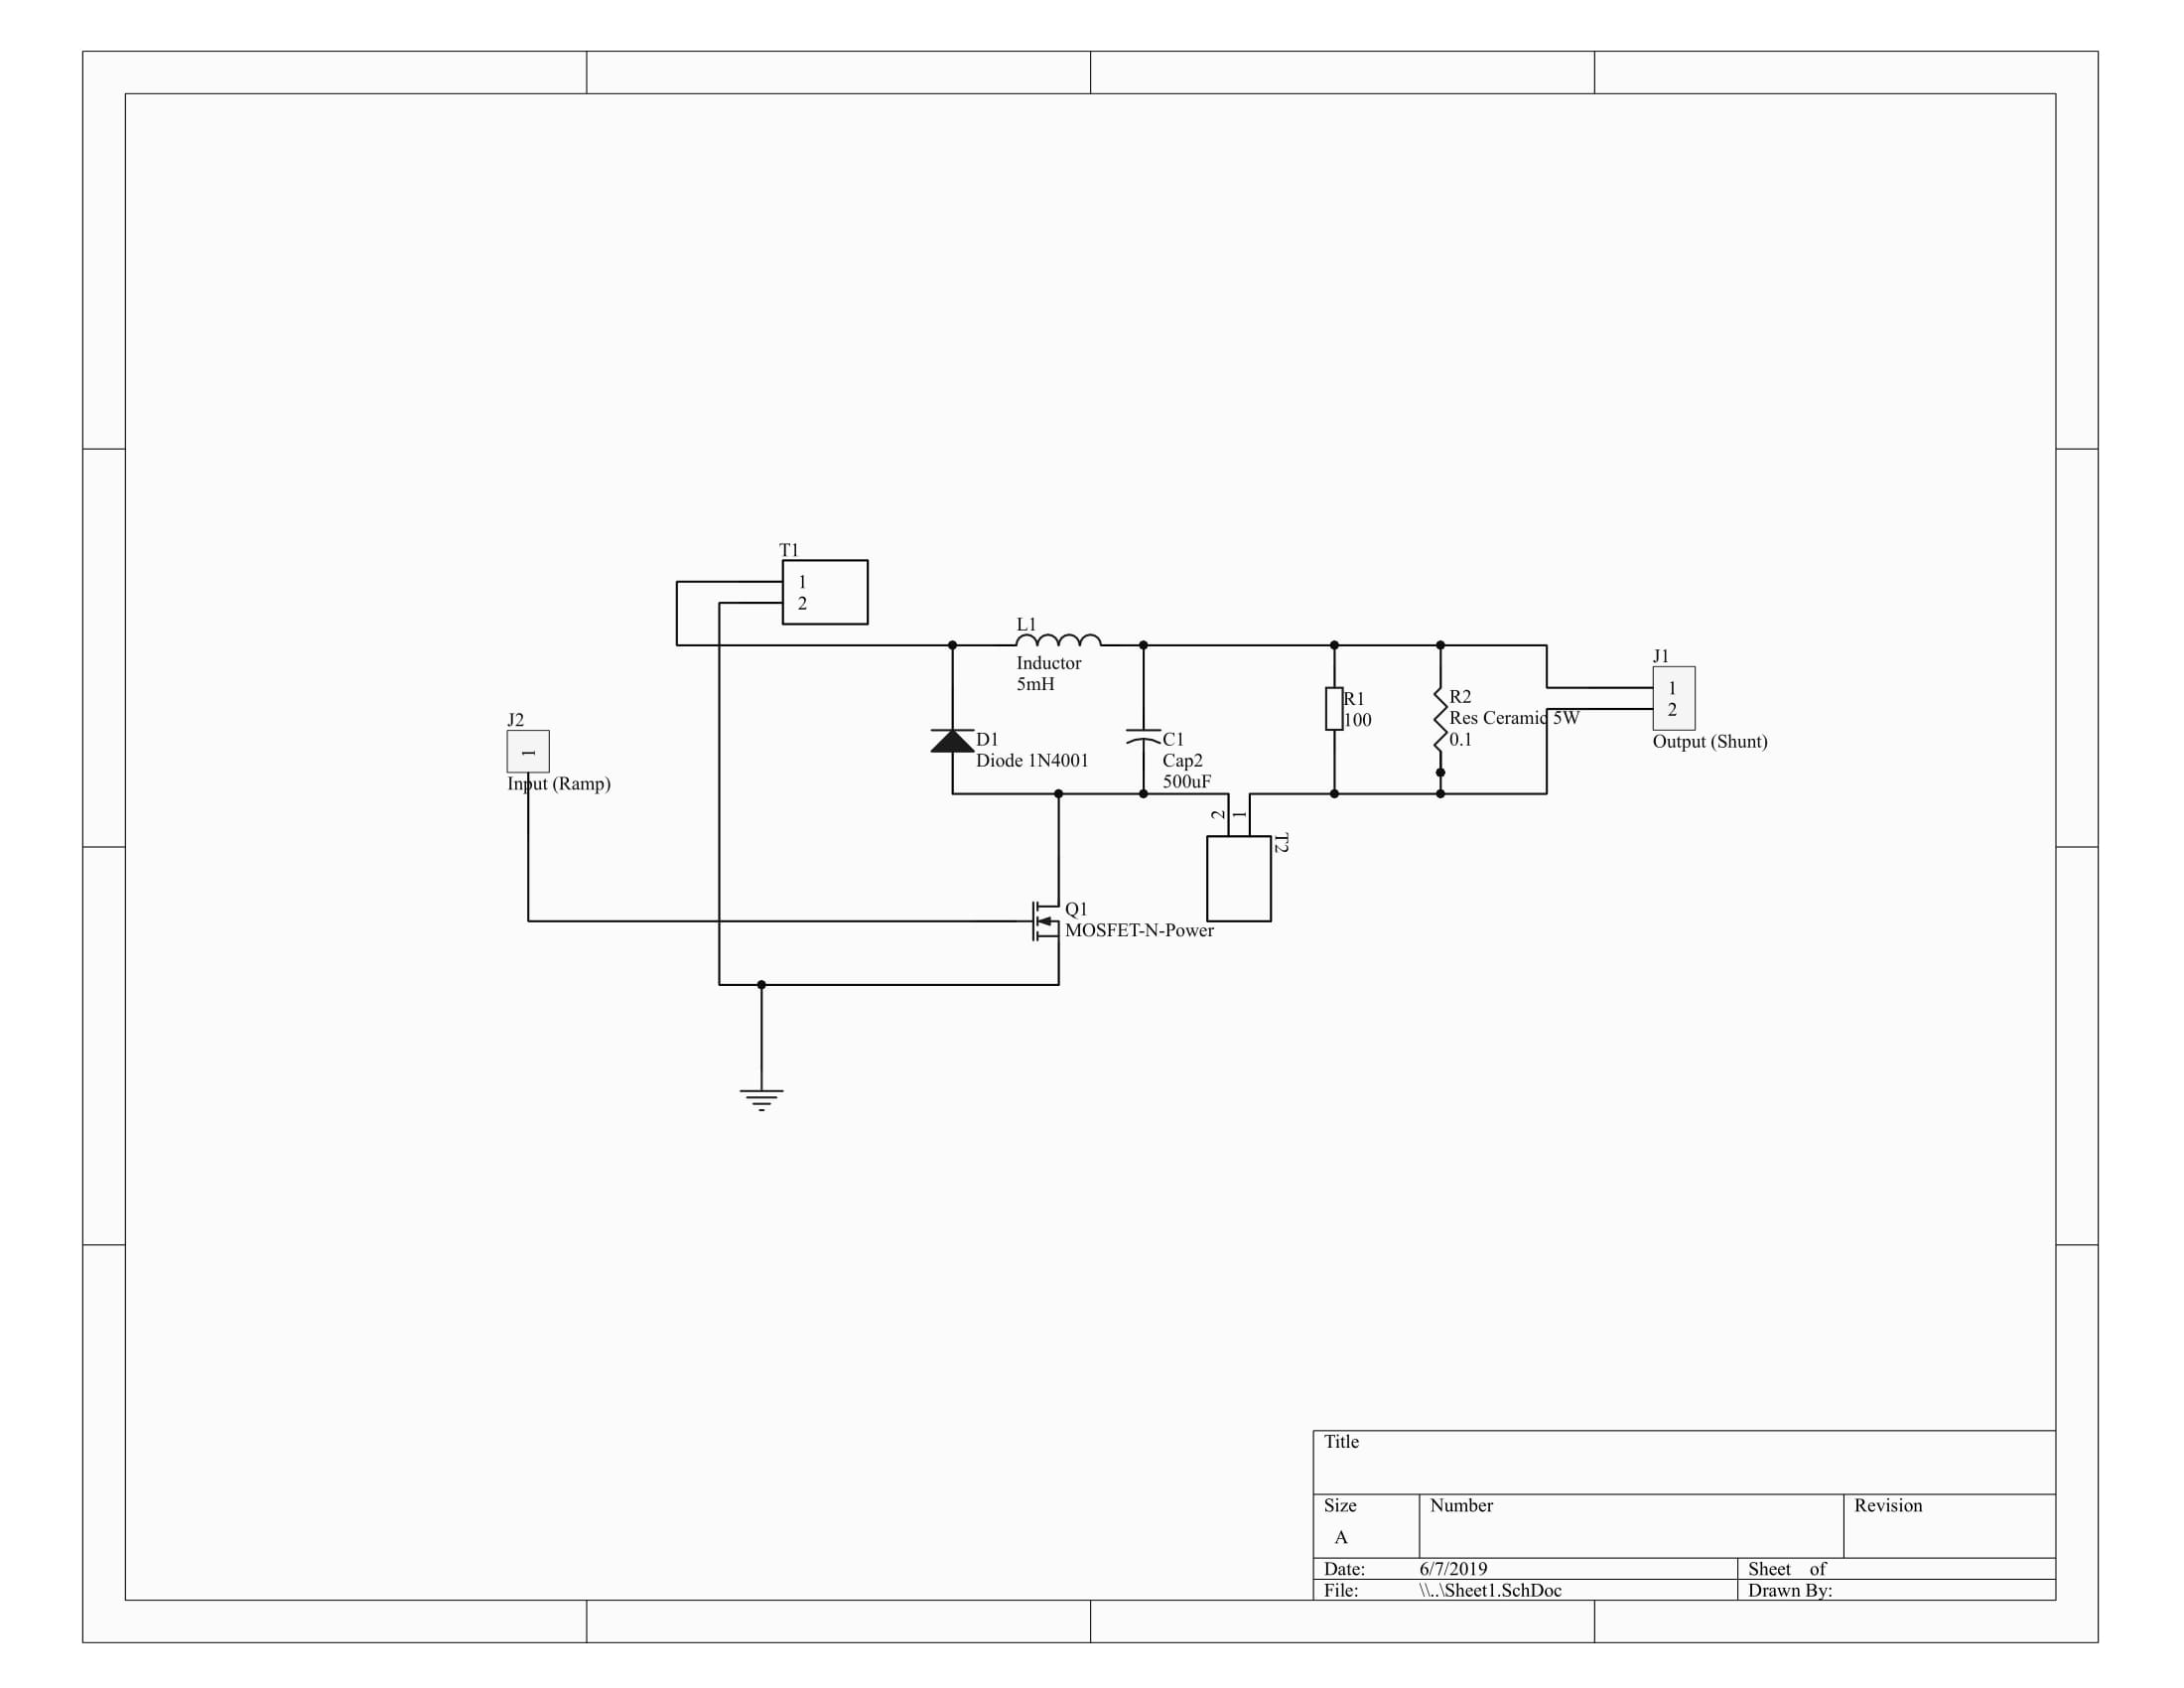
\includegraphics[angle=270,origin=c,scale=0.27]{Fig_05-1.jpg}
    \caption{Buck Converter Circuit}
    \label{fig:Buck Converter Circuit}
\end{figure}
\begin{figure}[H]
    \centering
    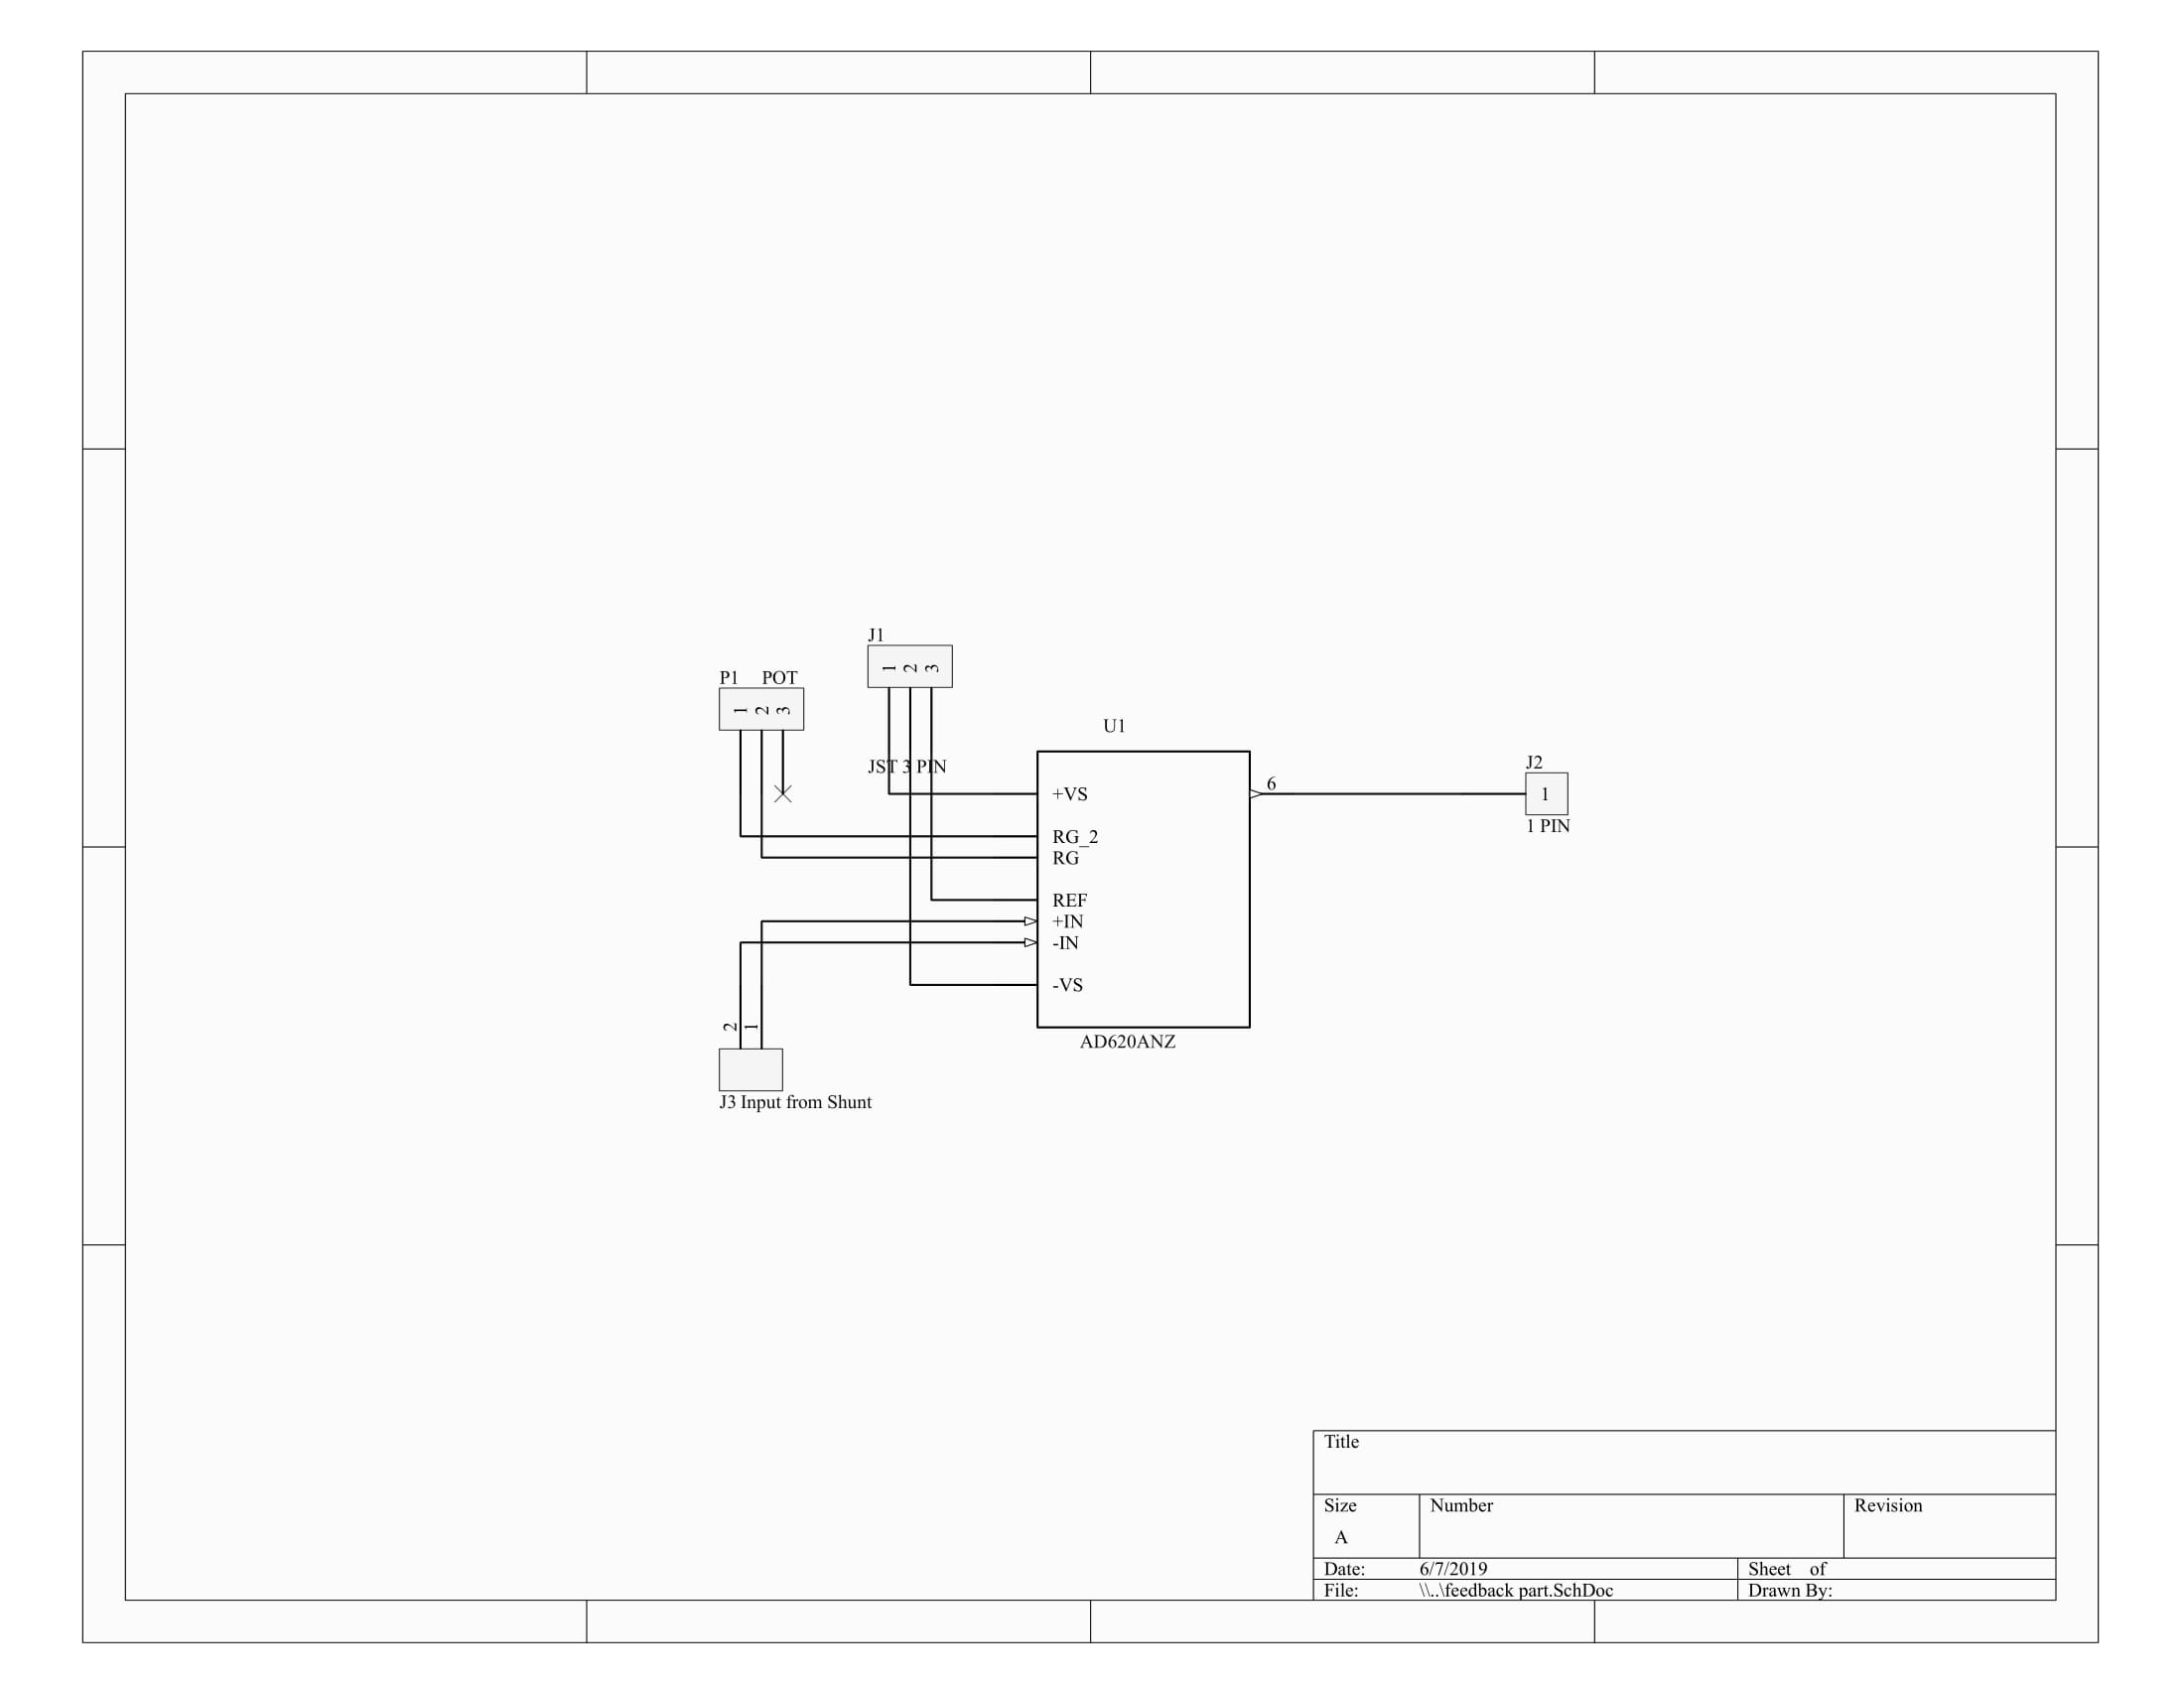
\includegraphics[angle=270,origin=c,scale=0.27]{Fig_06-1.jpg}
    \caption{Feedback Circuit}
    \label{fig:Feedback Circuit}
\end{figure}
\begin{multicols}{2}
\subsection{PCB Layouts}
\begin{figure}[H]
    \centering
    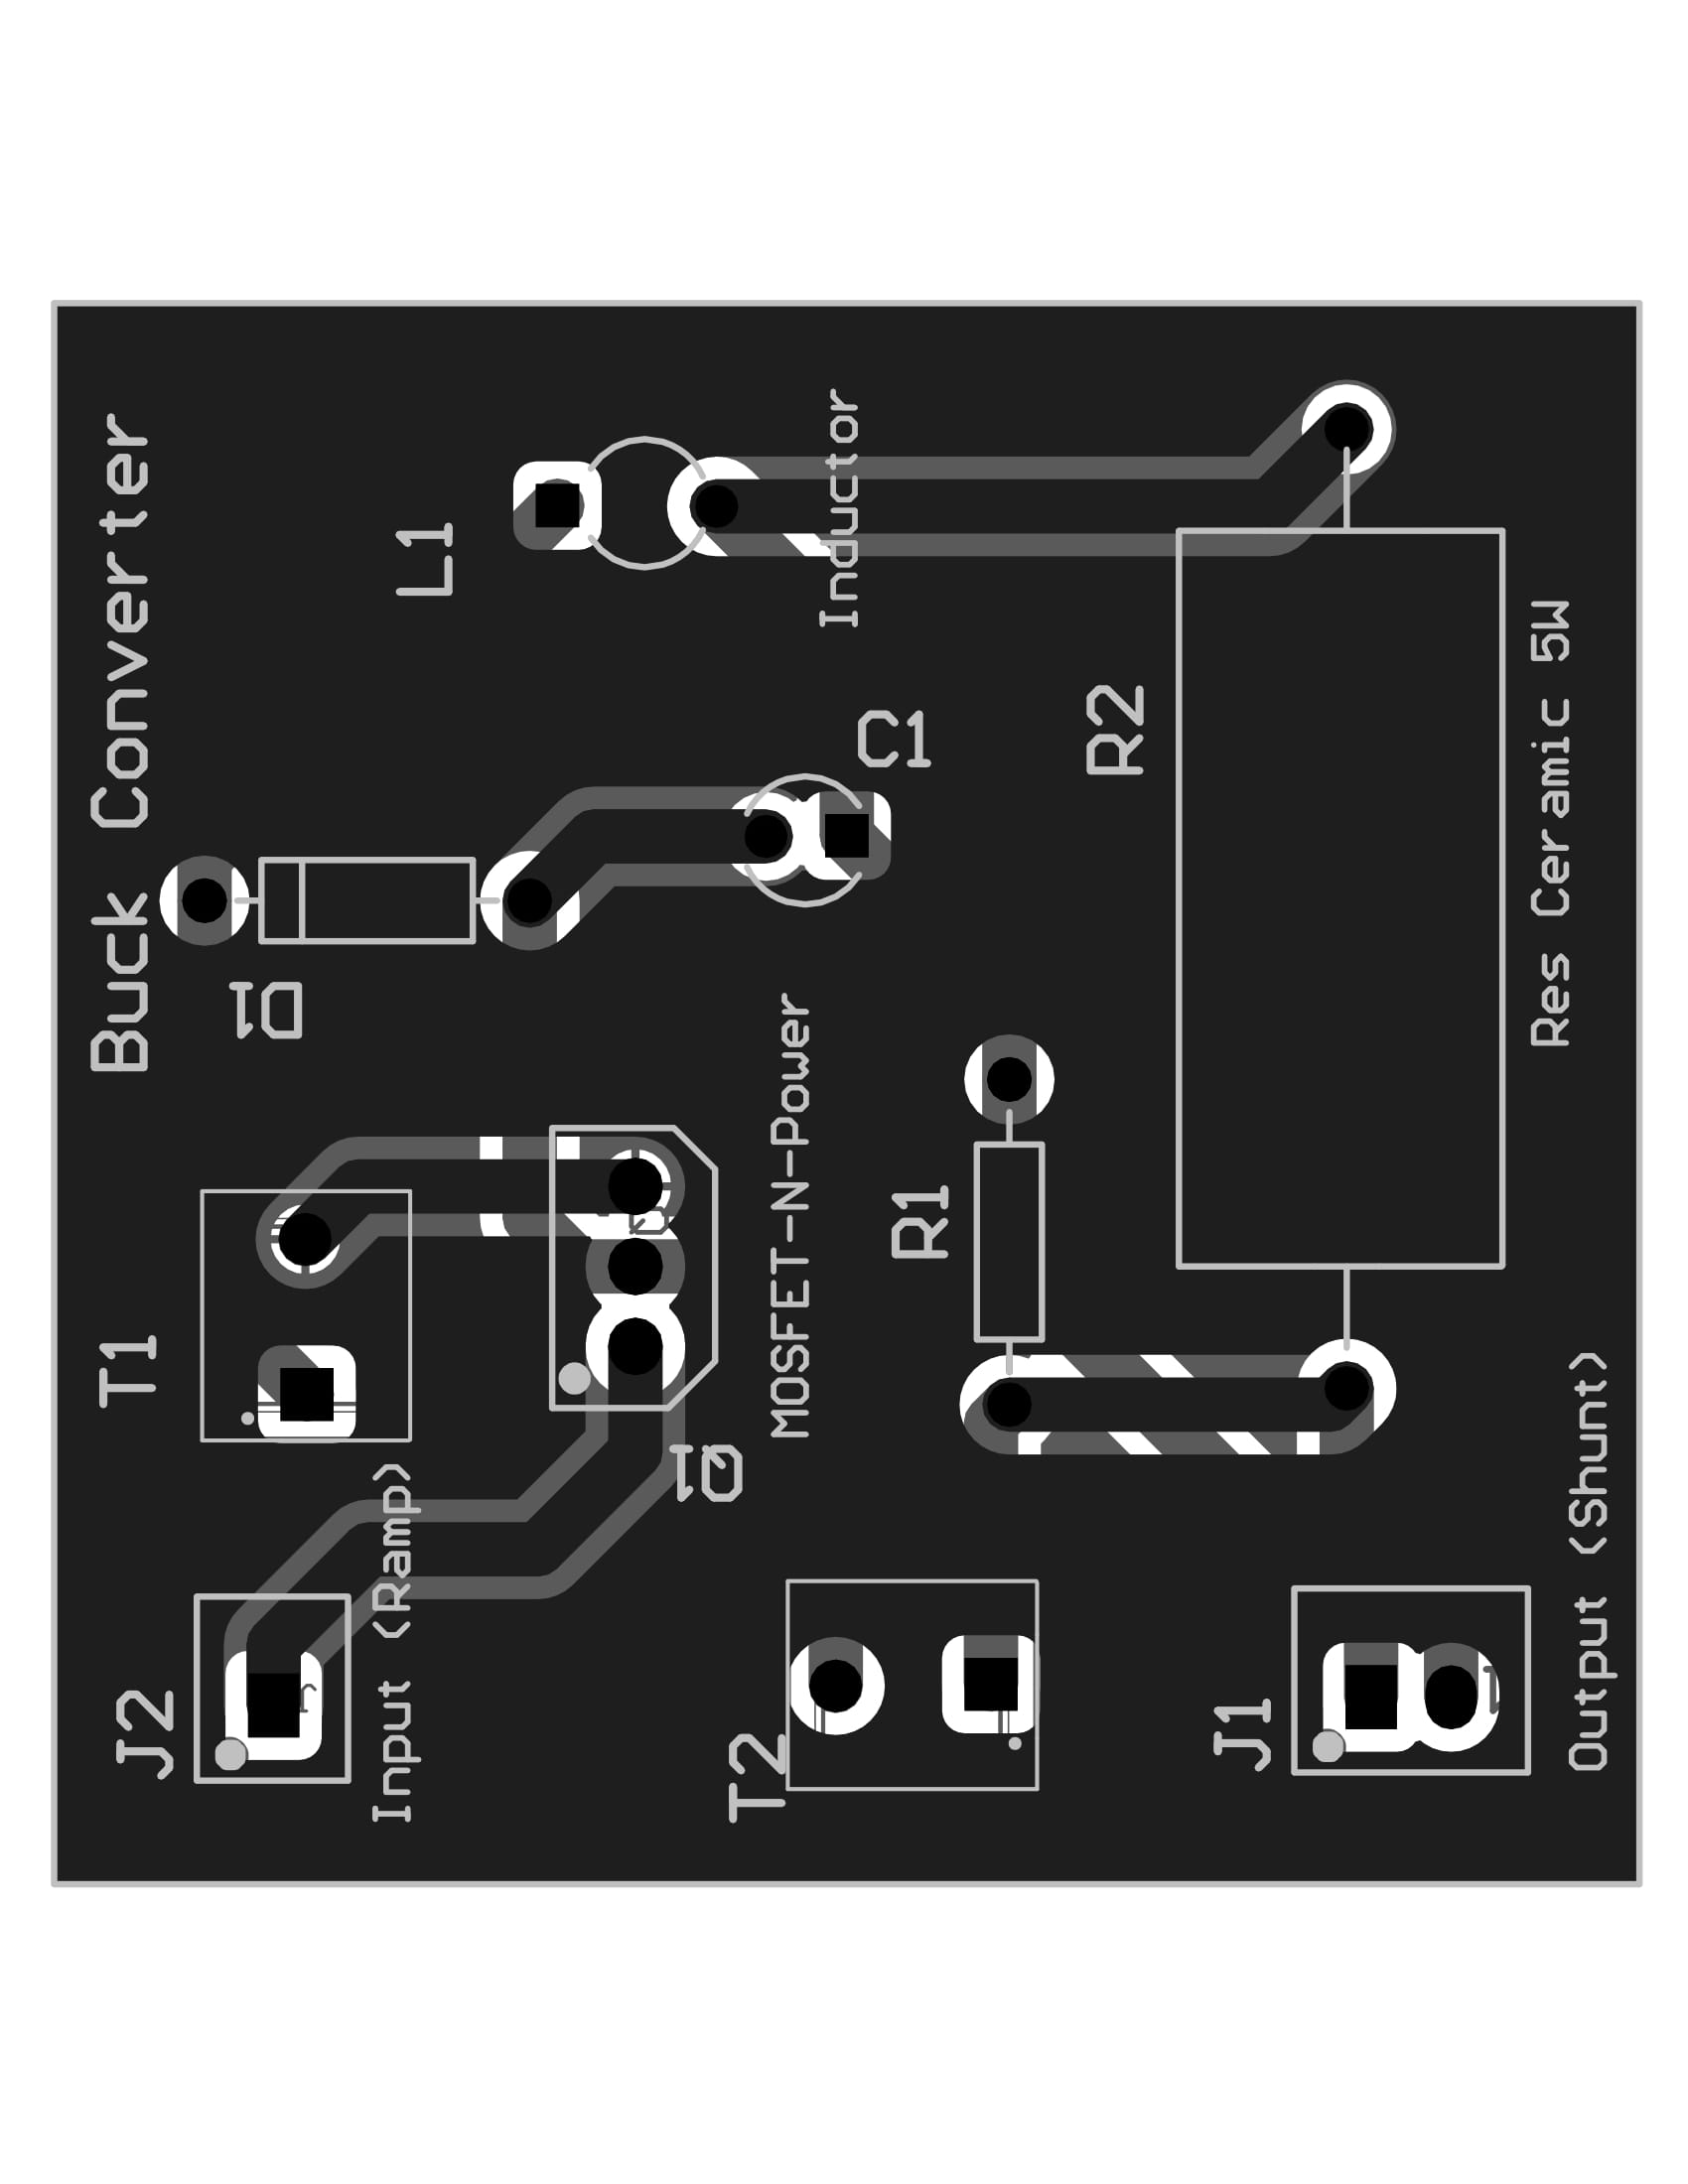
\includegraphics[width=7cm]{Fig_07-1.jpg}
    \caption{Buck Converter PCB Layout}
    \label{fig:Buck PCB}
\end{figure}
\begin{figure}[H]
    \centering
    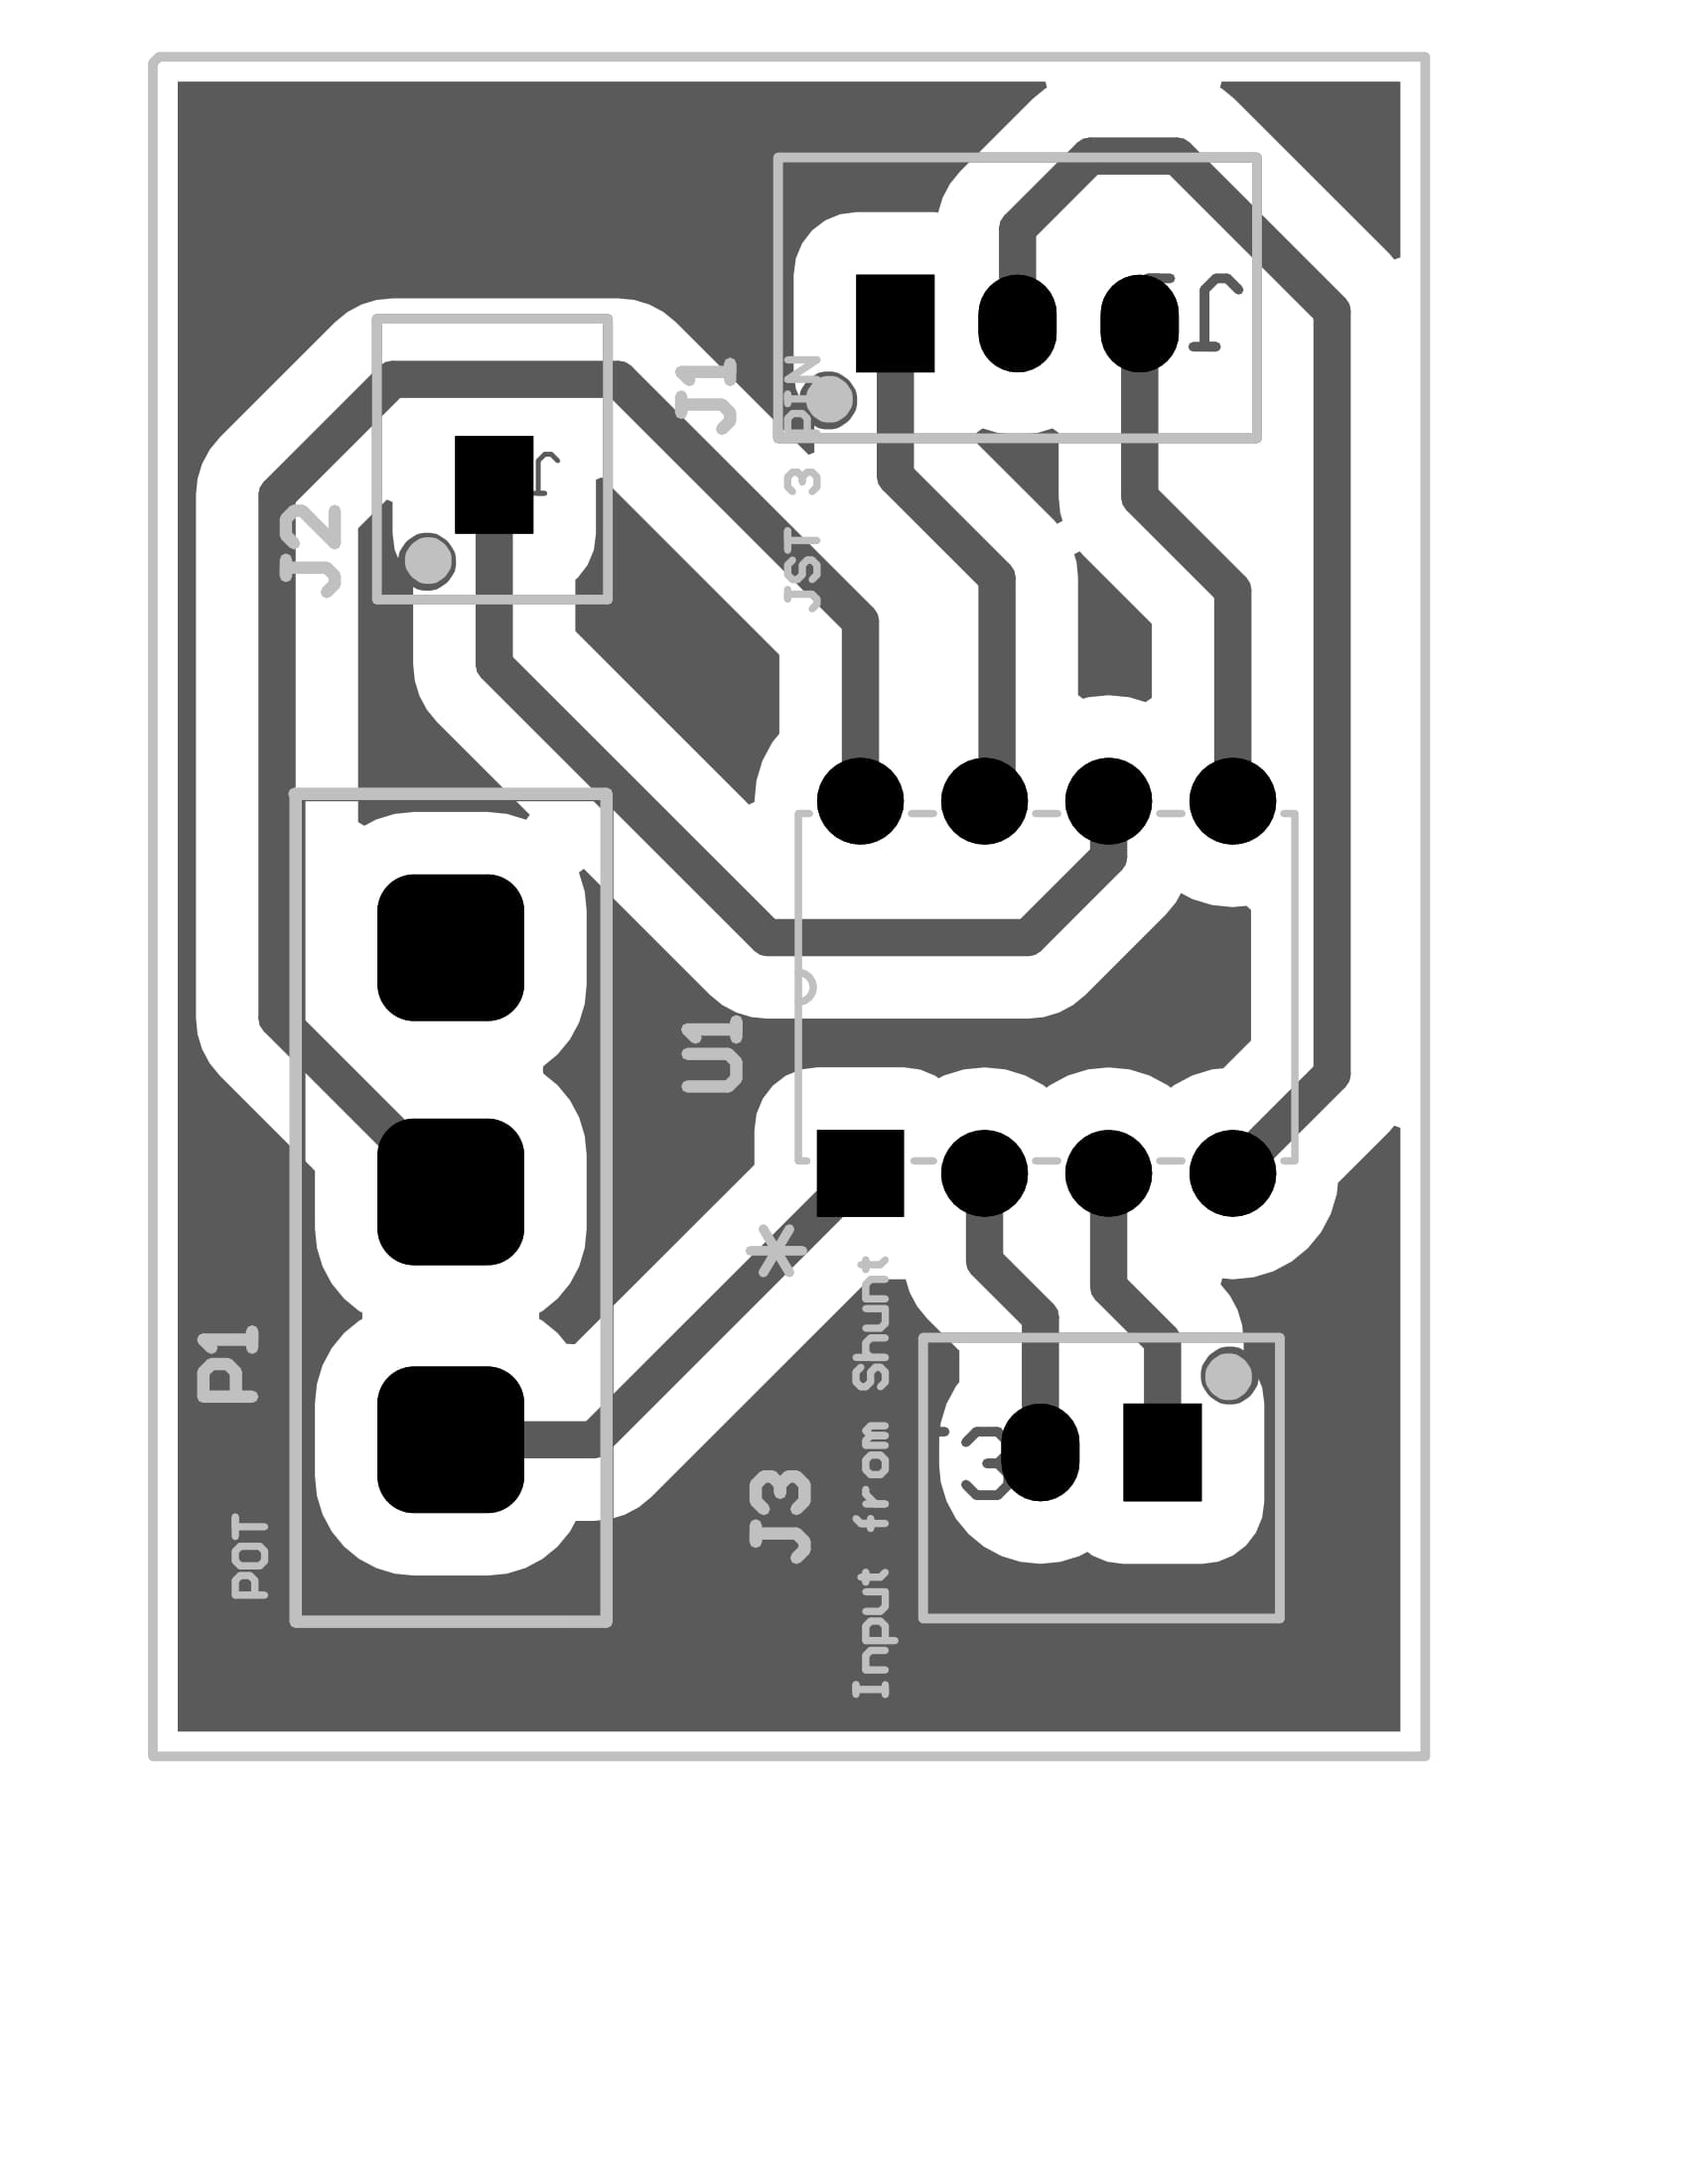
\includegraphics[width=7cm]{Fig_08-1.jpg}
    \caption{Amplifier PCB Layout}
    \label{fig:Amp PCB}
\end{figure}
\begin{figure}[H]
    \centering
    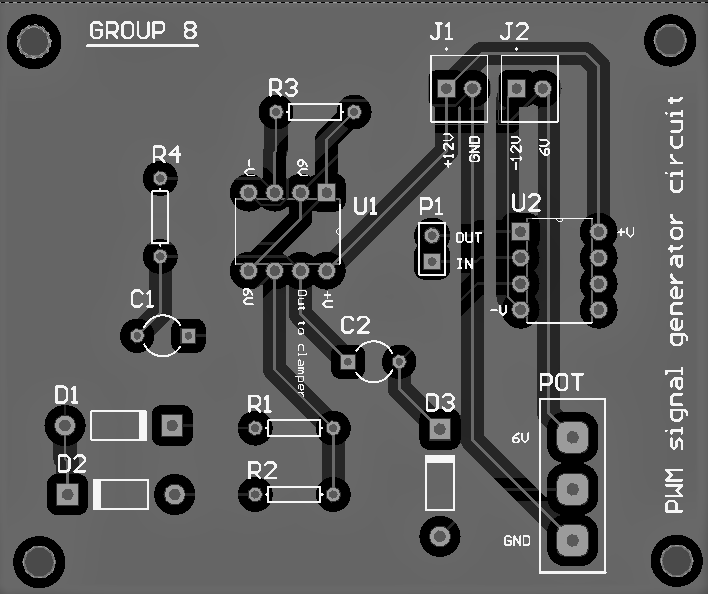
\includegraphics[width=7cm]{ramp_pcb.png}
    \caption{Ramp PCB Layout}
    \label{fig:Ramp PCB}
\end{figure}
\subsection{Enclosure Design}
\begin{figure}[H]
    \centering
    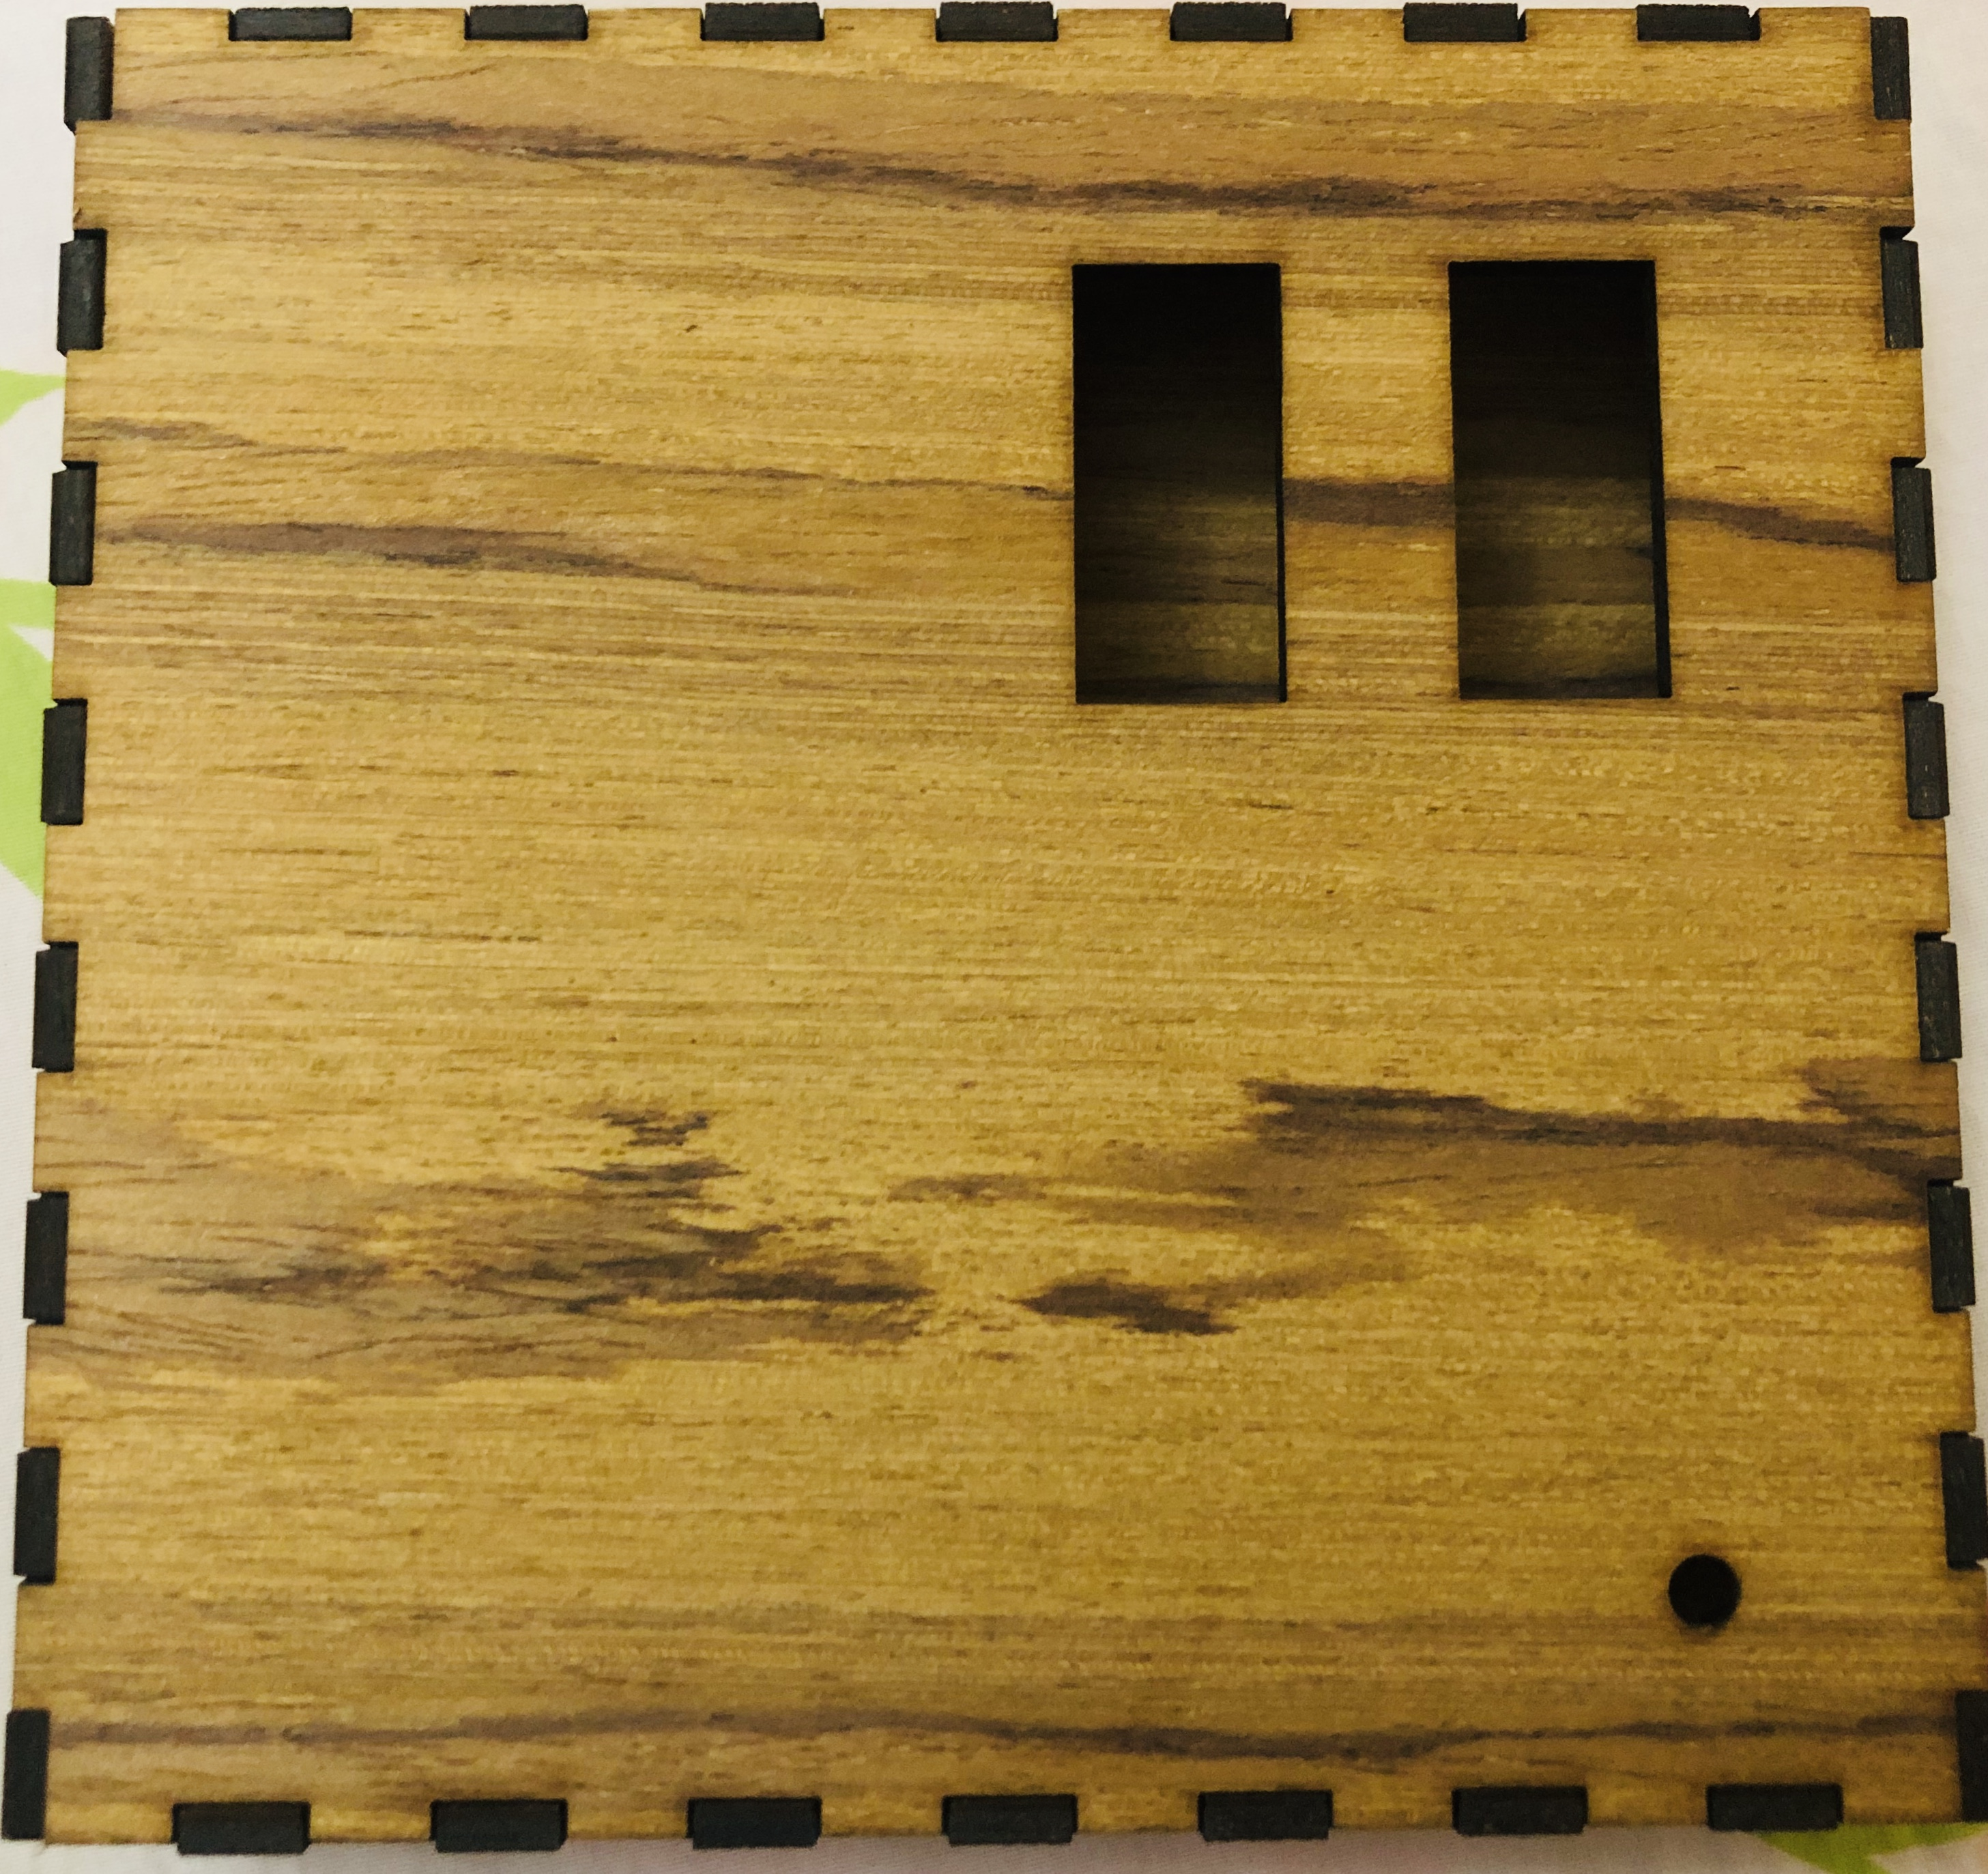
\includegraphics[width=7cm]{enclosure3.jpg}
    \caption{Enclosure Top}
    \label{fig:En Top}
\end{figure}
\begin{figure}[H]
    \centering
    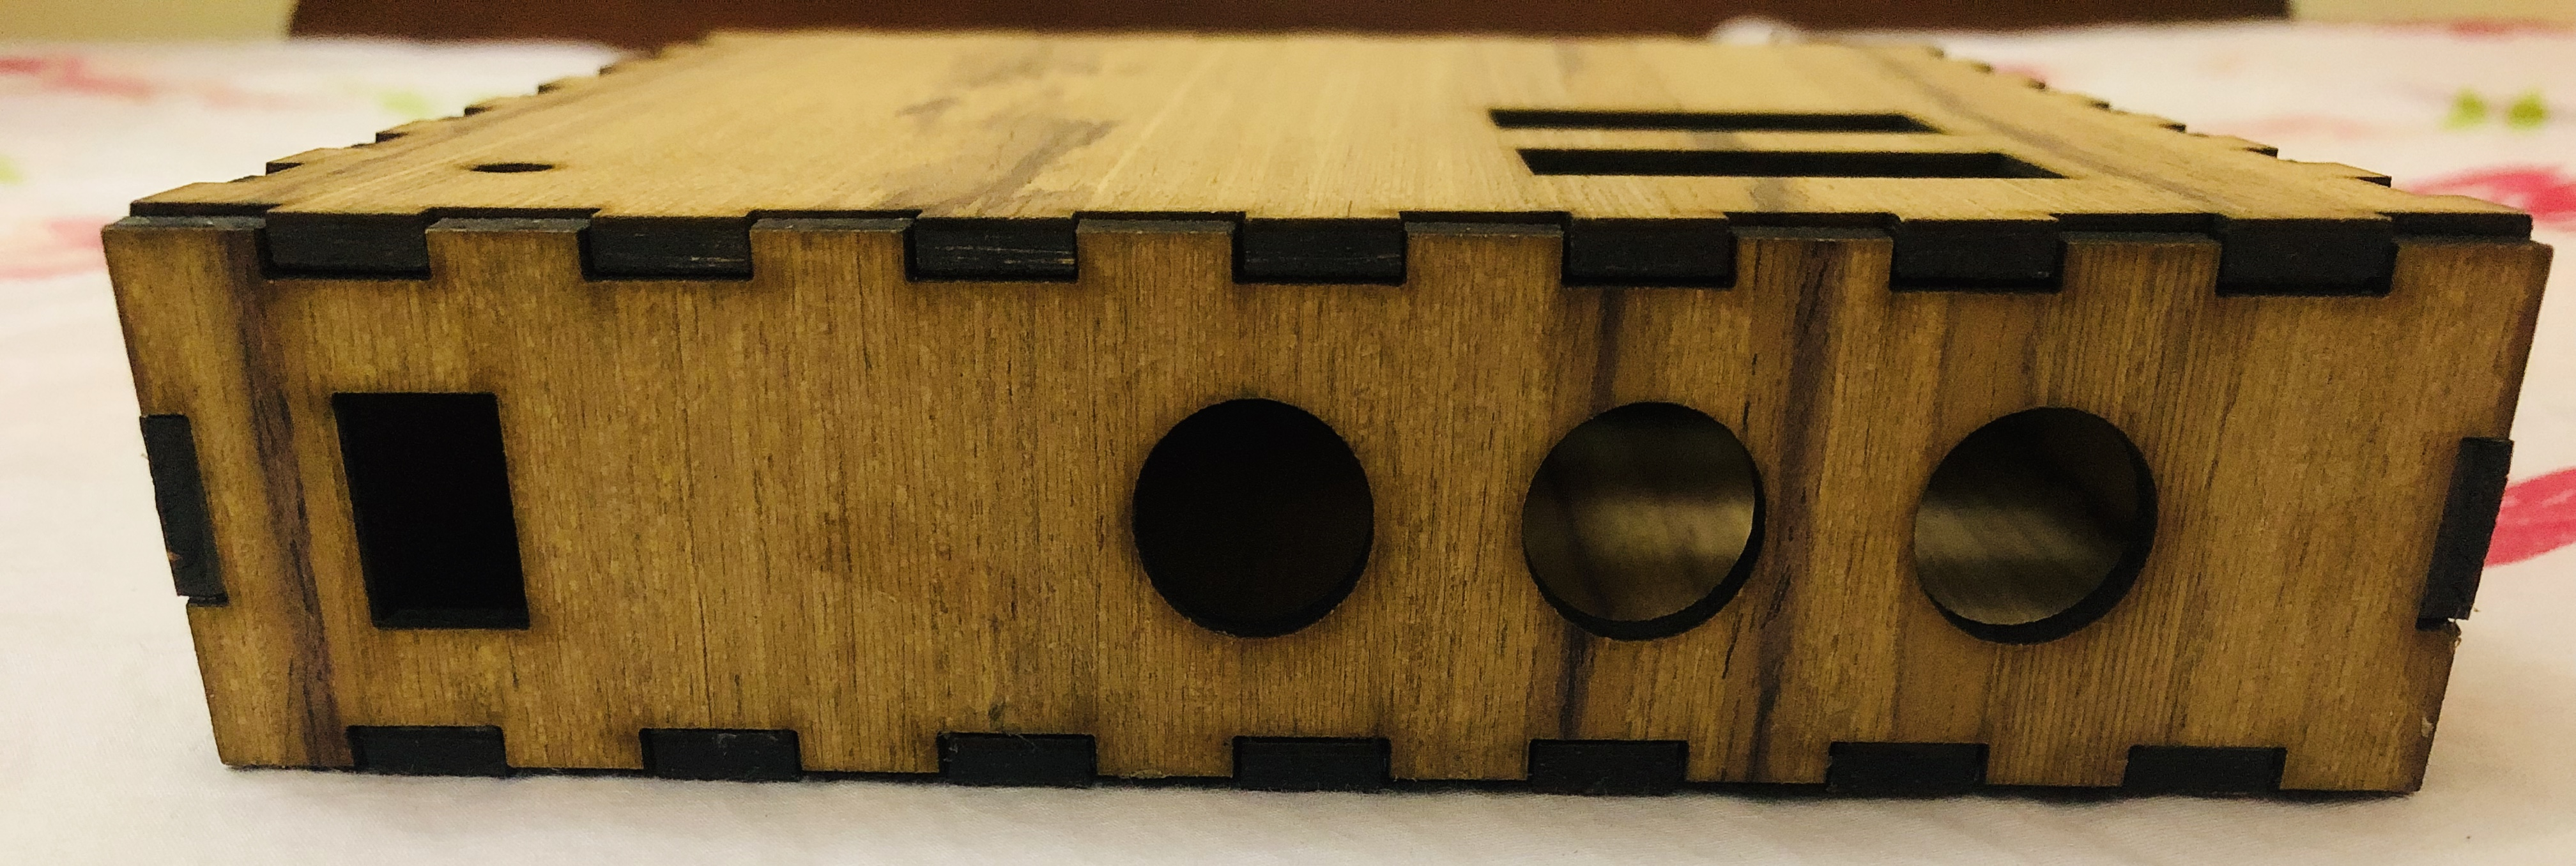
\includegraphics[width=7cm]{enclosure2.jpg}
    \caption{Enclosure Back}
    \label{fig:En back}
\end{figure}
\end{multicols}
\end{document}